% Options for packages loaded elsewhere
\PassOptionsToPackage{unicode}{hyperref}
\PassOptionsToPackage{hyphens}{url}
%
\documentclass[
]{article}
\usepackage{lmodern}
\usepackage{setspace}
\usepackage{amsmath}
\usepackage{ifxetex,ifluatex}
\ifnum 0\ifxetex 1\fi\ifluatex 1\fi=0 % if pdftex
  \usepackage[T1]{fontenc}
  \usepackage[utf8]{inputenc}
  \usepackage{textcomp} % provide euro and other symbols
  \usepackage{amssymb}
\else % if luatex or xetex
  \usepackage{unicode-math}
  \defaultfontfeatures{Scale=MatchLowercase}
  \defaultfontfeatures[\rmfamily]{Ligatures=TeX,Scale=1}
  \setmainfont[]{Arial}
\fi
% Use upquote if available, for straight quotes in verbatim environments
\IfFileExists{upquote.sty}{\usepackage{upquote}}{}
\IfFileExists{microtype.sty}{% use microtype if available
  \usepackage[]{microtype}
  \UseMicrotypeSet[protrusion]{basicmath} % disable protrusion for tt fonts
}{}
\makeatletter
\@ifundefined{KOMAClassName}{% if non-KOMA class
  \IfFileExists{parskip.sty}{%
    \usepackage{parskip}
  }{% else
    \setlength{\parindent}{0pt}
    \setlength{\parskip}{6pt plus 2pt minus 1pt}}
}{% if KOMA class
  \KOMAoptions{parskip=half}}
\makeatother
\usepackage{xcolor}
\IfFileExists{xurl.sty}{\usepackage{xurl}}{} % add URL line breaks if available
\IfFileExists{bookmark.sty}{\usepackage{bookmark}}{\usepackage{hyperref}}
\hypersetup{
  pdftitle={Investigating sex differences in genetic relatedness in great-tailed grackles in Tempe, Arizona to infer potential sex biases in dispersal},
  pdfauthor={Sevchik A1; Logan CJ2, 3; McCune KB3; Blackwell A4; Rowney C2; Lukas D2*},
  hidelinks,
  pdfcreator={LaTeX via pandoc}}
\urlstyle{same} % disable monospaced font for URLs
\usepackage[margin=1in]{geometry}
\usepackage{color}
\usepackage{fancyvrb}
\newcommand{\VerbBar}{|}
\newcommand{\VERB}{\Verb[commandchars=\\\{\}]}
\DefineVerbatimEnvironment{Highlighting}{Verbatim}{commandchars=\\\{\}}
% Add ',fontsize=\small' for more characters per line
\usepackage{framed}
\definecolor{shadecolor}{RGB}{248,248,248}
\newenvironment{Shaded}{\begin{snugshade}}{\end{snugshade}}
\newcommand{\AlertTok}[1]{\textcolor[rgb]{0.94,0.16,0.16}{#1}}
\newcommand{\AnnotationTok}[1]{\textcolor[rgb]{0.56,0.35,0.01}{\textbf{\textit{#1}}}}
\newcommand{\AttributeTok}[1]{\textcolor[rgb]{0.77,0.63,0.00}{#1}}
\newcommand{\BaseNTok}[1]{\textcolor[rgb]{0.00,0.00,0.81}{#1}}
\newcommand{\BuiltInTok}[1]{#1}
\newcommand{\CharTok}[1]{\textcolor[rgb]{0.31,0.60,0.02}{#1}}
\newcommand{\CommentTok}[1]{\textcolor[rgb]{0.56,0.35,0.01}{\textit{#1}}}
\newcommand{\CommentVarTok}[1]{\textcolor[rgb]{0.56,0.35,0.01}{\textbf{\textit{#1}}}}
\newcommand{\ConstantTok}[1]{\textcolor[rgb]{0.00,0.00,0.00}{#1}}
\newcommand{\ControlFlowTok}[1]{\textcolor[rgb]{0.13,0.29,0.53}{\textbf{#1}}}
\newcommand{\DataTypeTok}[1]{\textcolor[rgb]{0.13,0.29,0.53}{#1}}
\newcommand{\DecValTok}[1]{\textcolor[rgb]{0.00,0.00,0.81}{#1}}
\newcommand{\DocumentationTok}[1]{\textcolor[rgb]{0.56,0.35,0.01}{\textbf{\textit{#1}}}}
\newcommand{\ErrorTok}[1]{\textcolor[rgb]{0.64,0.00,0.00}{\textbf{#1}}}
\newcommand{\ExtensionTok}[1]{#1}
\newcommand{\FloatTok}[1]{\textcolor[rgb]{0.00,0.00,0.81}{#1}}
\newcommand{\FunctionTok}[1]{\textcolor[rgb]{0.00,0.00,0.00}{#1}}
\newcommand{\ImportTok}[1]{#1}
\newcommand{\InformationTok}[1]{\textcolor[rgb]{0.56,0.35,0.01}{\textbf{\textit{#1}}}}
\newcommand{\KeywordTok}[1]{\textcolor[rgb]{0.13,0.29,0.53}{\textbf{#1}}}
\newcommand{\NormalTok}[1]{#1}
\newcommand{\OperatorTok}[1]{\textcolor[rgb]{0.81,0.36,0.00}{\textbf{#1}}}
\newcommand{\OtherTok}[1]{\textcolor[rgb]{0.56,0.35,0.01}{#1}}
\newcommand{\PreprocessorTok}[1]{\textcolor[rgb]{0.56,0.35,0.01}{\textit{#1}}}
\newcommand{\RegionMarkerTok}[1]{#1}
\newcommand{\SpecialCharTok}[1]{\textcolor[rgb]{0.00,0.00,0.00}{#1}}
\newcommand{\SpecialStringTok}[1]{\textcolor[rgb]{0.31,0.60,0.02}{#1}}
\newcommand{\StringTok}[1]{\textcolor[rgb]{0.31,0.60,0.02}{#1}}
\newcommand{\VariableTok}[1]{\textcolor[rgb]{0.00,0.00,0.00}{#1}}
\newcommand{\VerbatimStringTok}[1]{\textcolor[rgb]{0.31,0.60,0.02}{#1}}
\newcommand{\WarningTok}[1]{\textcolor[rgb]{0.56,0.35,0.01}{\textbf{\textit{#1}}}}
\usepackage{longtable,booktabs}
\usepackage{calc} % for calculating minipage widths
% Correct order of tables after \paragraph or \subparagraph
\usepackage{etoolbox}
\makeatletter
\patchcmd\longtable{\par}{\if@noskipsec\mbox{}\fi\par}{}{}
\makeatother
% Allow footnotes in longtable head/foot
\IfFileExists{footnotehyper.sty}{\usepackage{footnotehyper}}{\usepackage{footnote}}
\makesavenoteenv{longtable}
\usepackage{graphicx}
\makeatletter
\def\maxwidth{\ifdim\Gin@nat@width>\linewidth\linewidth\else\Gin@nat@width\fi}
\def\maxheight{\ifdim\Gin@nat@height>\textheight\textheight\else\Gin@nat@height\fi}
\makeatother
% Scale images if necessary, so that they will not overflow the page
% margins by default, and it is still possible to overwrite the defaults
% using explicit options in \includegraphics[width, height, ...]{}
\setkeys{Gin}{width=\maxwidth,height=\maxheight,keepaspectratio}
% Set default figure placement to htbp
\makeatletter
\def\fps@figure{htbp}
\makeatother
\setlength{\emergencystretch}{3em} % prevent overfull lines
\providecommand{\tightlist}{%
  \setlength{\itemsep}{0pt}\setlength{\parskip}{0pt}}
\setcounter{secnumdepth}{-\maxdimen} % remove section numbering
\usepackage[left]{lineno}
\linenumbers
\ifluatex
  \usepackage{selnolig}  % disable illegal ligatures
\fi
\newlength{\cslhangindent}
\setlength{\cslhangindent}{1.5em}
\newlength{\csllabelwidth}
\setlength{\csllabelwidth}{3em}
\newenvironment{CSLReferences}[2] % #1 hanging-ident, #2 entry spacing
 {% don't indent paragraphs
  \setlength{\parindent}{0pt}
  % turn on hanging indent if param 1 is 1
  \ifodd #1 \everypar{\setlength{\hangindent}{\cslhangindent}}\ignorespaces\fi
  % set entry spacing
  \ifnum #2 > 0
  \setlength{\parskip}{#2\baselineskip}
  \fi
 }%
 {}
\usepackage{calc}
\newcommand{\CSLBlock}[1]{#1\hfill\break}
\newcommand{\CSLLeftMargin}[1]{\parbox[t]{\csllabelwidth}{#1}}
\newcommand{\CSLRightInline}[1]{\parbox[t]{\linewidth - \csllabelwidth}{#1}\break}
\newcommand{\CSLIndent}[1]{\hspace{\cslhangindent}#1}

\title{Investigating sex differences in genetic relatedness in
great-tailed grackles in Tempe, Arizona to infer potential sex biases in
dispersal}
\author{Sevchik
A\textsuperscript{1} \and \href{http://CorinaLogan.com}{Logan
CJ}\textsuperscript{2},
\textsuperscript{3} \and \href{https://www.kelseymccune.com}{McCune
KB}\textsuperscript{3} \and \href{https://blackwell-lab.com}{Blackwell
A}\textsuperscript{4} \and Rowney
C\textsuperscript{2} \and \href{http://dieterlukas.strikingly.com}{Lukas
D}\textsuperscript{2}*}
\date{2021-03-03}

\begin{document}
\maketitle

\setstretch{1.2}
\hypertarget{affiliations}{%
\subparagraph{Affiliations:}\label{affiliations}}

\begin{enumerate}
\def\labelenumi{\arabic{enumi})}
\tightlist
\item
  Arizona State University, 2) Max Planck Institute for Evolutionary
  Anthropology, 3) University of California Santa Barbara, 4) Washington
  State University, *Corresponding author:
  \href{mailto:dieter.lukas@eva.mpg.de}{\nolinkurl{dieter.lukas@eva.mpg.de}}
\end{enumerate}

~ ~ \textbf{The preregistration for this study has been pre-study peer
reviewed and received an In Principle Recommendation by:}

\includegraphics[width=0.25\textwidth,height=\textheight]{logoPCIecology.png}

Sophie Beltran-Bech (2019 In Principle Acceptance) Investigate fine
scale sex dispersal with spatial and genetic analyses. \emph{Peer
Community in Ecology}, 100036.
\href{https://doi.org/10.24072/pci.ecology.100036}{10.24072/pci.ecology.100036}.
Reviewers: Sylvine Durand and one anonymous reviewer

~

\hypertarget{abstract}{%
\subsection{Abstract}\label{abstract}}

In most bird species, females disperse prior to their first breeding
attempt, while males remain closer to the place they hatched for their
entire lives. Explanations for such female bias in natal dispersal have
focused on the resource-defense based monogamous mating system that is
prevalent in most birds. In this system, males are argued to benefit
from philopatry because knowing the local environment can help them to
establish territories to attract females, while females are argued to
benefit from dispersing because they can find suitable unrelated mates.
However, theoretical, field, and comparative studies highlight that the
factors shaping dispersal decisions are often more complex. Studying
species with different social and mating systems can help illuminate the
relative role of various factors in the evolution of sex biased
dispersal. Here, we use genetic approaches to determine whether females
and/or males disperse in great-tailed grackles (\emph{Quiscalus
mexicanus}), which have a mating system where the males hold breeding
territories that multiple females might choose to place their nest in,
but females forage independently of these breeding territories across a
wider area. First, we find that, for individuals caught at a single site
in Arizona, the average relatedness among all female dyads is higher
than average relatedness among other individuals at the site, whereas
average relatedness among all males dyads is not. Second, we find that
female close relatives are found within shorter distances from each
other than pairs of unrelated females, whereas male close relatives are
found at larger distances from each other than pairs of unrelated males.
Third, we find a decline in relatedness with increasing spatial
distances for females, but not for males. Our results indicate sex
biases in relatedness structure that differ from most other bird
species. Female great-tailed grackles associate with close genetic
relatives, presumably by remaining close to where they hatched which
would lead to them remaining close to their mothers and sisters. Males
are not found close to genetic relatives, suggesting that they disperse
away from their fathers and brothers. Our findings show that
great-tailed grackles offer a relevant study system to further
understand the factors shaping natal philopatry and dispersal, given
this reversal of the usual sex-bias in dispersal in line with their
divergent social and mating system.

\newpage

\hypertarget{introduction}{%
\subsection{Introduction}\label{introduction}}

Maturing birds face a decision about where to establish themselves for
breeding. In the majority of avian species, the potential costs and
benefits of breeding movement decisions appear to differ between the
sexes, with males remaining in the area they hatched while females move
to breed elsewhere (Greenwood 1980). The main theory proposed to explain
this sex bias towards male philopatry has focused on the
resource-defense based monogamous mating system found in most bird
species (Greenwood 1980; Trochet et al. 2016). In monogamous systems,
males tend to stay philopatric to defend an area they know to provide
resources to attract females, whereas females disperse to avoid the risk
of inbreeding with close relatives who dominate reproduction in the
area. However, alternative hypotheses about the benefits and costs of
philopatry or dispersal could equally apply to explain the dominant
female bias in dispersal among species with resource defense based
monogamy. In general, it is likely that, in both sexes, decisions of
whether to remain in the area or to move short or substantial distances
to new breeding grounds are influenced by an interplay of the potential
costs of movement, resource availability and competition, and the
potential benefits or costs of interacting with close relatives (Mabry
et al. 2013; Trochet et al. 2016; Li and Kokko 2019). One way toward a
better understanding of the relative role of the various factors that
potentially explain breeding movement decisions of both female and male
birds is to study dispersal in species with different social and mating
systems.

Studying dispersal outside of well established study systems is
difficult, which means that there is only limited information from bird
species with unusual social and mating systems. It is challenging to set
up studies that span a large geographical area where the identity of
many individuals can be established and followed. As such, the fate of
individuals who leave the area often remains unknown and it is unclear
whether new individuals found in the area have moved to the area or were
simply not observed previously (Walters 2000). To overcome these
challenges, genetic approaches are now incorporated to identify
dispersal patterns (Lawson Handley and Perrin 2007; Banks and Peakall
2012). In particular, to identify potential sex biases in dispersal, two
approaches are used. The first approach relies on determining the
spatial distribution of variants of genetic markers that have a
sex-specific inheritance (Lawson Handley and Perrin 2007). The second
approach uses data from a large number of genetic markers spread across
the genome to determine how the similarity across these markers changes
with increasing spatial distances among males and females (Banks and
Peakall 2012). Studies based on the second approach have increased in
recent years because the costs of generating genotypes for a large
sample of individuals have rapidly decreased (Harrison, York, and Young
2014; Weinman, Solomon, and Rubenstein 2015; and Thrasher et al. 2018).

Here, we investigate SNP (single nucleotide polymorphism) genotype data
for a sample of great-tailed grackle (\emph{Quiscalus mexicanus})
females and males at a single site. Great-tailed grackles differ in
several aspects from the majority of bird species in which dispersal has
been investigated thus far, which might make them a relevant study
system to gain further insights into the factors shaping the dispersal
decisions of females and males. Great-tailed grackles are a highly
social passerine bird found in the Americas. Individuals forage
year-round in small fission-fusion groups in areas that are not
obviously defended against other individuals and at night they roost in
large associations (Johnson and Peer 2001), unlike most other bird
species where, at least during the breeding season, pairs or families
defend foraging territories (Cockburn 2006). This could indicate that
resource competition might be lower in great-tailed grackles,
potentially reducing pressure to remain in or move to high quality
areas. Essentially everywhere they occur, great-tailed grackles live in
human-modified environments (MacGregor-Fors et al. 2009) and their wide
range of foraging habits routinely includes exploiting human foods (King
2012). In these environments, they can occur in large numbers and at
high densities (Escobar-Ibáñez, Rueda-Hernández, and MacGregor-Fors
2020). Great-tailed grackles have recently extensively expanded their
geographic range (Wehtje 2003), indicating that they are highly mobile.
Great-tailed grackles are sexually dimorphic, with males being larger
than females and differing in plumage. During the mating season, some
males defend territories around suitable breeding habitats and mate with
females who build their nests in these territories. Holding a territory
leads to higher reproductive success for these males, but females also
mate with roaming males, leading to a polygamous mating system (Johnson
et al. 2000). This resembles the mating system observed in many
mammalian species, where males disperse to areas with the highetst
number of potential mates (e.g. Höner et al. 2007). Previously,
great-tailed grakckle females were assumed to perform all activities
related to offspring care, from building the nest through incubating and
feeding the hatchlings, but observations indicate that at least some
males partake in these activities (Selander 1970; Folsom et al. 2020).
Both the mating and the social system are accordingly different from the
resource-defense based monogamous system found in the majority of birds,
which might lead to a deviation from female-biased dispersal.
Determining patterns of philopatry and dispersal in great-tailed
grackles can offer further insights into the potential association
between dispersal decisions and the various factors that might shape
them.

\hypertarget{hypotheses}{%
\subsection{Hypotheses}\label{hypotheses}}

Our main hypothesis assumes that great-tailed grackles show a pattern of
female-bias in dispersal. It is our main hypothesis because this
dispersal pattern predominates across birds and dispersal patterns are
often retained from a common ancestor; in addition, the factors that
shape this pattern might still operate in great-tailed grackles. Our
alternative hypotheses expect that some of the differences in the social
and mating system of great-tailed grackles might lead to a deviation
from this dispersal pattern. We set these as alternative hypotheses
because it is still unclear which factors might be important and if they
might be of importance in a particular species. With the setup of our
study, we cannot infer why or how dispersal patterns might have changed,
therefore we present these hypotheses simply as alternatives.

\textbf{Hypothesis} There are sex differences in the natal disperal rate
and distance among individuals in great-tailed grackles (\emph{Quiscalus
mexicanus}) with males remaining close to where they hatched and females
moving away from where they hatched. Males are expected to remain close
to the area where they hatched, therefore a large number of the males on
the Arizona State University (ASU) campus are expected to have hatched
within the area of the study site and stay close to their relatives. In
contrast, females are expected to move before their first breeding
attempt (Greenwood 1980), therefore females on campus are likely to come
from areas outside of campus in the surrounding area, having moved away
from relatives.

\textbf{Alternative hypothesis 1} Males disperse away from where they
hatched, while females remain where they hatched.

\textbf{Alternative hypothesis 2} Individuals of both sexes remain close
to where they hatched.

\textbf{Alternative hypothesis 3} Individuals of both sexes disperse
away from where they hatched.

We expect that the movement of individuals will influence the spatial
distribution of genetic relatives (Aguillon et al. 2017). Individuals of
the sex that remains close to where they hatched are expected to be
close to genetic relatives, while individuals of the sex that disperses
are expected to be more distant from genetic relatives. We also expect
that the further the distance an individual moves, the less likely they
are to be even distantly related to another individual within the study
area. Our hypotheses generate specific predictions about contrasts in
the levels of relatedness and the spatial distribution of genetic
relatives according to whether individuals are philopatric or disperse.
The first analysis (analysis i: average levels of relatedness among
individuals in our sample) focuses on whether individuals disperse
beyond the trapping area and compares one average value of relatedness
per sex. Here, we predict higher levels of average relatedness among all
individuals of the philopatric sex than among all individuals of the sex
that disperses. This follows if some dispersing emigrants move outside
of the trapping area, away from parents and siblings, while immigrants
can come from a variety of areas outside of the trapping area and
therefore consist of unrelated individuals. The second analysis
(analysis ii: geographic distances between individuals that are close
genetic relatives) focuses on the distances among close relatives of the
same sex that are trapped within our trapping area and investigates the
pairwise distances among individuals of the same sex who are closely
related. Here, we predict that there are sex biases in the average
distances between trapping sites for relatives compared to non-relatives
because philopatric individuals will remain close to same-sex parents
and siblings while indiivduals that disperse within the trapping area
will end up in different locations than their same-sex parents and
siblings. The third analysis (analysis iii: spatial autocorrelation)
focuses on how relatedness among pairs of same sex individuals changes
as the distance between them increases and investigates correlations
among all estimates of pairwise relatedness and pairwise geographic
distances among individuals of the same sex. Here, we predict a decline
in levels of relatedness as distances among individuals increase to
indicate that individuals have remained philopatric such that close
relatives are found in close geographic proximity. In contrast, we
predict no structure of relatedness in geographic space for individuals
who disperse because relatives will be found both close and far from
each other.

\hypertarget{deviations-from-the-preregistration}{%
\subsection{Deviations from the
preregistration}\label{deviations-from-the-preregistration}}

We preregistered our hypotheses, methods, and analysis plans. Analyses
began in March 2020 after the preregistration passed pre-study peer
review at \emph{Peer Community In Ecology} in November 2019. The final
version of the preregistration can be found here
\url{http://corinalogan.com/Preregistrations/gdispersal.html}.

We made the following changes and additions to the analyses (explained
in detail in the Methods section below):\\
- we adjusted the sample to exclude juveniles and reflect sex
composition\\
- we used a more stringent filter for the ddRadSeq single nucleotide
polymorphism\\
- we excluded one genotype with implausible levels of heterozygosity\\
- we chose the Queller \& Goodnight estimator to calculate pairwise
relatedness\\
- we added an analysis to assess whether the geographic distances among
closely related females were shorter than those in a random sample of
females\\
- we added a configuration to the spatial correlogram analyses, based on
the observed distances among related individuals

\newpage

\hypertarget{methods}{%
\subsection{Methods}\label{methods}}

The methods below are based on the preregistration, with small changes
summarized in the
\protect\hyperlink{deviations-from-the-preregistration}{Deviations from
the preregistration} section above and further explained here (in
italics).

\hypertarget{data}{%
\subsubsection{Data}\label{data}}

\hypertarget{sample}{%
\paragraph{Sample}\label{sample}}

DNA from 57 great-tailed grackles was obtained from wild individuals
caught in Tempe, Arizona, USA (see Figure 4 for a map showing the trap
locations and sample sizes for the individuals included in the
analyses). These individuals were either immediately released, or
temporarily brought into aviaries for behavioral testing and then
released back to the wild.

\emph{Deviation from preregistration: During the preparation of the
analyses, we noticed that we made a mistake when calculating the sex
composition in the sample: different from what was written in the
preregistration, the sample for our genetic analyses consists of 41 (not
40) females and 16 (not 17) males. In addition, we realized that the
sample included some juvenile individuals (\textless1 yr of age). We
excluded these four juveniles from the main analyses because they might
have been pre-dispersal at the time of capture. In addition, we excluded
one individual after genotyping (see below). The dataset for the all
analyses therefore consisted of 37 adult females and 15 adult males.}

\includegraphics{gdispersal_Fig3_samplesites.png} \textbf{Figure 1.} Map
displaying the sampling locations of grackles on the Arizona State
University campus and the number of great-tailed grackles trapped at
each location as part of this research.

The larger number of females than males in our sample appears to reflect
the adult sex ratio at this study site. To estimate the sex ratio at the
field site, we counted the number of females and males that were trapped
in mist nets since the beginning of our study (September 2017 - October
2019). This trapping method likely does not elicit a sex bias in terms
of which sex is caught because the nets are invisible. Therefore, if one
sex is more neophobic than the other, both sexes are likely to be
trapped using this method. A total of 26 females and 11 males were
trapped using mist nets (a ratio of 2.36 females per 1 male), which is
very similar to the sex ratio in our sample consisting of 37 adult
females and 15 adult males (2.47 females per 1 male).

Females were caught at all but one site, such that comparisons are
possible of the genetic relatedness of pairs of females trapped at
various distances from each other. Males were not caught at all trap
sites, but there are several sites at which multiple males were caught
and sufficient sites for comparisons of males that were caught close to
each other, and at intermediate and large distances from each other.

\hypertarget{sample-size-rationale}{%
\paragraph{Sample size rationale}\label{sample-size-rationale}}

The sample size presented was the largest one possible (due to the time
required for trapping) by July 2019 when the DNA were sequenced using
ddRADseq.

\hypertarget{data-collection-stopping-rule}{%
\paragraph{Data collection stopping
rule}\label{data-collection-stopping-rule}}

We analyzed all blood samples that were collected through June 2019,
which was the end of the trapping season.

\hypertarget{open-data}{%
\paragraph{Open data}\label{open-data}}

All data necessary for the analyses are available at
\url{https://doi.org/10.5063/F1W66J48} (Lukas 2020) and at GitHub (the
code included in the R markdown file will load these files directly from
GitHub). The raw genetic data is available at
\url{https://www.ncbi.nlm.nih.gov/sra?term=SRP278340}.

\hypertarget{randomization-and-counterbalancing}{%
\paragraph{Randomization and
counterbalancing}\label{randomization-and-counterbalancing}}

No randomization or counterbalancing is involved in this study.

\hypertarget{blinding-of-conditions-during-analysis}{%
\paragraph{Blinding of conditions during
analysis}\label{blinding-of-conditions-during-analysis}}

Experimenters were blind to the sex of the bird when processing samples
using ddRADseq (only the alphanumeric bird ID was visible on the tube
and no team member who handled the samples memorized which ID goes with
which bird because we give the birds names).

\hypertarget{blood-collection}{%
\paragraph{Blood collection}\label{blood-collection}}

Whole blood samples were collected from individual birds by brachial or
medial metatarsal venipuncture. Blood was collected and stored in one of
two ways until DNA extraction:

\begin{enumerate}
\def\labelenumi{\arabic{enumi})}
\item
  At the beginning of the project (2018), 70uL of whole blood was added
  to silicone-coated micro-blood collection tubes containing 280uL of
  lysis buffer (White and Densmore 1992, 50--51) and stored at room
  temperature for up to a year before DNA extraction.
\item
  In 2018 a different method was implemented, using DNA from packed red
  blood cells: 150uL of blood was collected from trapped great-tailed
  grackles and stored for a minimum of 30 minutes and a maximum of 60
  minutes at room temperature or 3 hours on ice. Samples were then
  centrifuged at 15x gravity for 10 minutes to separate the serum from
  the cellular fraction. After the serum layer was removed and stored,
  600uL lysis buffer (White and Densmore 1992, 50--51) was added to the
  remaining packed cells. Tubes containing packed cells and lysis buffer
  were stored at room temperature for up to 1 year before extraction.
\end{enumerate}

\hypertarget{dna-extraction-and-quantification}{%
\paragraph{DNA extraction and
quantification}\label{dna-extraction-and-quantification}}

Some samples were extracted at Arizona State University by Rowney
(samples through Dec 2018), while others were shipped with ice packs to
Washington State University for extraction by Blackwell and his lab
(samples collected Jan-Jun 2019). DNA was extracted from the above
samples using the DNeasy Blood and Tissue kit (Qiagen) with slight
modifications from the manufacturer's protocol (see details in Thrasher
et al. (2018) Supporting Information, page 7). Approximately 100ul of
blood/lysis mixture was mixed with 20ul Proteinase K, 150ul PBS, and
200ul buffer AL, then incubated overnight at 64C while shaking. Samples
were mixed with 200ul ethanol and added to spin columns. Columns were
centrifuged and washed according to kit protocol using buffers AW1 and
AW2. DNA was eluted into 50ul of RNAse and DNAse free water at 64C after
a 5-10 min incubation on columns. DNA quantification was then performed
on a Qubit 4.0 Fluorometer (Fisher Scientific) following the
manufacturer's protocol for broad range dsDNA. The average yield of
samples used for sequencing was 34ng/ul. Extracted DNA samples were
shipped with ice packs to the Cornell Lab of Ornithology for ddRAD
sequencing in July 2019.

\hypertarget{ddrad-sequencing}{%
\paragraph{ddRAD sequencing}\label{ddrad-sequencing}}

We generated single-nucleotide polymorphism (SNP; where at a given
position in the genome two different bases, alleles, can occur)
genotypes for 57 individuals from our study site in Arizona (we excluded
the above mentioned 5 individuals later). The DNA was processed using
ddRADseq by Sevchik and Bronwyn Butcher (Cornell University) following
methods in Thrasher et al. (2018). Each of the samples' DNA
concentrations was measured using the Qubit dsDNA BR Assay Kit and the
Qubit Fluorometer following the manufacturer's protocol. For this
particular experiment, the necessary DNA concentrations were between
5-50ng/ul and so any sample outside of this range needed to be
normalized. Those samples with a concentration higher than 50ng/ul were
diluted to approximately 25ng/ul with nuclease-free water. For those
samples with concentrations lower than 5ng/ul, both elutions were pooled
and the DNA concentrated by evaporation using an Eppendorf Vacufuge. The
DNA extracts are then run through a PCR thermocycler where the fragments
are digested with a combination of two restriction enzymes (SbfI-HF and
MspI) and 20 different adapters attached to the end of the DNA pieces. A
1\% agarose gel is run to ensure the proper digestion and ligation of
the DNA samples. The samples are then cleaned up using MagNA beads and
size selected using BluePippin for a prespecified length (between
400-700 base pairs). After the samples return from size selection, they
are amplified using a low-cycle PCR process and pooled together to be
sent in to be sequenced. Sequencing was performed on an Illumina
NextSeq500 (using a mid-output kit and run with Illumina PhiX control
(15\%) to aid sequence alignment) to generate 150 bp single end reads at
the Core Facilities of the Cornell Institute of Biotechnology.

\hypertarget{snp-processing}{%
\paragraph{SNP processing}\label{snp-processing}}

These data were post-processed to generate SNP data for relatedness
analyses as in Thrasher et al. (2018). After filtering reads for quality
and demultiplexing to assign sequences back to specific individuals,
genetic loci were assembled \emph{de novo} because no reference genome
exists for great-tailed grackles.

\emph{Deviation from preregistration: For the ddRadSeq single nucleotide
polymorphism (SNP) filtering, two sets of restrictions were applied to
maximize power by focusing the analysis on the most informative SNPs
while reducing the potential risk of noise. The first filter was based
on the parameters set forth by Thrasher et al. (2018), which they showed
to provide a set of loci with strong power to discern relationships
among individuals. Loci were only considered if they were present in
80\% of the samples (r parameter of the stacks pipeline) and had a
minimum frequency of the minor allele of 0.05 (min maf parameter of the
stacks pipeline). This meant that the rare variant at a locus was
present in at least 5\% of the samples and it resulted in 3647
acceptable SNPs for analyses. The second filter applied more stringent
conditions for the loci to be retained. Loci were only considered if
they were present in 95\% of the samples (r) and had a minimum minor
allele frequency of 0.05 (min maf). This resulted in 635 acceptable
SNPs; 3012 SNPs fewer than in the first, less restrictive filtering, but
still more than in the study by Thrasher et al. (2018) because each
individual in our sample had been sequenced to a greater depth. We
decided to use the resulting genotypes from the second, more restrictive
setting for the relatedness analyses because of our small sample size
(e.g., if some individuals had a lower quality sample, their relatedness
to other individuals might consistently be misclassified) and because
these settings still provided an effective number of SNPs for analyses.
The more restrictive filtering reduces noise from missing data and
retains high power by selecting loci with high heterozygosity (their
heterozygosity approaches the maximum of 0.5) {[}Morin et al.~2004{]}.}

\emph{Addition to preregistration: The preregistration had focused on
analyses to address the hypotheses. We realized that we should also
provide descriptive statistics of the genotype data we generated
specificially for this study. We used functions in the R packages
`adegenet' (Jombart 2008), `pegas' (Paradis 2010), and `popgenutils
(Tourvas 2020) to edit the genotype data and to calculate, based on the
allele frequencies in the data and assuming random mating, the expected
heterozygosity (average chance of finding two different alleles across
loci across individuals) and probability of identity (chance that two
individuals will have the same set of alleles across all loci).}

\hypertarget{relatedness-estimation}{%
\paragraph{Relatedness estimation}\label{relatedness-estimation}}

Genetic relatedness between all pairs of individuals was calculated
using the package ``related'' (Pew et al. 2015) in R, following methods
in Thrasher et al. (2018). We used the frequencies of the alleles at the
generated SNPs to calculate relatedness among pairs of individuals, with
individuals being classified as related if they share more alleles than
what is expected based on random chance given the frequencies of
variants in the population (relatedness (R) \textgreater0) and as
unrelated if they share as many (R=0) or fewer genetic variants than
expected (R\textless0). We planned to use the function
`compareestimators' to assess which relatedness estimator appears to
perform the best given the characteristics of our data.

\emph{Deviation from preregistration: The `compareestimator' function in
the R package `related' caused fatal errors on multiple computers. We
therefore calculated pairwise relatedness using two estimators: 1) the
Wang estimator (Wang 2002), following the observation in Thrasher et al.
(2018) of the suitability of this estimator for ddRadSeq data, and 2)
the Queller-Goodnight estimator (Queller and Goodnight 1989), which is
the standard in several studies. With both sets of relatedness
estimates, all of our inferences (high levels of average relatedness
among females, shorter distances among closely related females, spatial
structure among female genotypes) were similar. We present the results
based only on the estimator by Queller \& Goodnight (1989) because we
noticed that, with our data, the estimator by Wang (2002) appeared to be
more influenced by missing data in the genotypes. We calculated average
relatedness between all pairs of individuals within one sex: the
arithmetic mean of the estimated relatedness based on sharing of SNP
alleles among all female dyads and all male dyads.}

\emph{Additional note: Our preregistration did not include plans to
perform pedigree reconstructions as an alternative way to assess
relatedness among the individuals for three reasons. First, we have a
cross-sectional sample, which does not contain longitudinal information
from tracking juveniles seen with their potential parents into
adulthood. Second, adults are of unknown age, so for any related
individuals who share an allele at (almost) all loci we would not be
able to determine which is the parent and which is the offspring. Third,
grackles are not expected to have large clusters of siblings (Johnson et
al. 2000), as for example in fish species, making it highly unlikely
that our sample contains extended families.}

\hypertarget{additional-variables}{%
\paragraph{Additional variables}\label{additional-variables}}

\begin{enumerate}
\def\labelenumi{\arabic{enumi})}
\item
  Sex (female, male): the sex of the individuals assigned based on
  morphological features
\item
  Distance between trap sites (meters): straight line distance (assuming
  earth is an ellipsoid) between all pairs of trapping locations based
  on the longitude and latitude of each site.
\end{enumerate}

\hypertarget{analyses}{%
\subsubsection{Analyses}\label{analyses}}

Analyses were conducted in R (current version 4.0.3; R Core Team
(2017)).

We did not plan to exclude any data. We did not have to exclude
individuals because more than half of their genotype was unknown.

\emph{Deviation from preregistration: After obtaining the SNP data, we
noticed that one individual, female A053PS, was indicated to be related
to all other individuals in the sample. When we checked the genotype of
this individual, it had much higher levels of heterozygosity,
independent of how we filtered the data. The genotype did not show signs
of shifting of alleles between loci (e.g., showing a genotype that lists
allele 2 from locus 1 with allele 1 from locus 2) or have issues with
missing data or the dropout of alleles. Instead, the increase in
heterozygosity was always close to the square of the heterozygosity
observed among the remaining individuals, suggesting that this genotype
might be constructed from two different individuals. We were not able to
retrace where such an error might have been introduced, therefore we
decided to exclude individual A053PS from the analyses.}

\hypertarget{ability-to-detect-actual-effects}{%
\paragraph{\texorpdfstring{\emph{Ability to detect actual
effects}}{Ability to detect actual effects}}\label{ability-to-detect-actual-effects}}

Birds the size of a grackle (\textasciitilde100-150 grams) are expected
to show a median natal dispersal distance of about 250-300 meters
(Sutherland et al. 2000). Our 15 trap locations were located within a
\textasciitilde1000m radius circle, suggesting that if there are
dispersers in our sample, these individuals will have most likely come
from areas outside of the trapping circle. In turn, if individuals
remain close to their natal area, they would only move distances much
shorter than this, suggesting that the pairwise distances between
non-dispersed relatives would be shorter than the random distance
between any two birds we caught. However, we do not know the average
distance that either philopatric or dispersing individuals move. The
scale of our sampling area might be so small that individuals of the sex
that disperses the least are likely to have hatched outside of this
area. In addition, there could be variation among either females or
males in the distances individuals move, with potentially also a small
proportion of individuals of the predominantly philopatric sex
dispersing, which could obscure patterns in the small sample of
individuals in our study. Accordingly, we might not be able to detect
differences in average relatedness between females and males (analysis
i), but we still might expect a sex bias in the geographic distances
among relatives (analysis ii).

We restricted our sample to adults to focus on the distribution of
individuals after any potential natal dispersal (Goudet, Perrin, and
Waser 2002). We only have individuals from within a single site, so we
did not use methods that rely on assigning individuals to a source
population or measure the relative distribution of genetic variation
within versus among populations (Fst or similar measures). We therefore
relied on measuring genetic relatedness between pairs of individuals.
Approaches relying on spatial analyses of multi-locus genotypes have
been shown to be able to detect even modest sex biased dispersal in
fine-scale spatial distribution, in particular analyses of spatial
autocorrelation (Banks and Peakall 2012). However, our sample size is
small, meaning that we might have only limited power to detect potential
differences between females and males (Goudet, Perrin, and Waser 2002).
For the spatial distribution of relatives (Analysis ii), the number of
related individuals in our sample might be too small to detect a strong
pattern of the relatives of one sex being more geographically closer to
each other than relatives of the other sex. For the
isolation-by-distance leading to a change in relatedness within the
range of our sampling locations, the signal might be too weak in either
or both sexes to make inferences about sex differences (Analysis iii).
However, for the comparison of average relatedness (Analysis i), given
that we have a large number of SNP loci, we expect that we should have
sufficient power to obtain a qualitative assessment of whether relatives
are present in our sample (Wang and Santure 2009) and accordingly
whether dispersal is more prevalent in either females or males. Examples
of empirical studies that detected a signal with small sample sizes
include Hofmann et al. (2012); Quaglietta et al. (2013); Gour et al.
(2013); and Botero-Delgadillo et al. (2017).

\hypertarget{analysis-i-average-relatedness-and-sex}{%
\paragraph{\texorpdfstring{\emph{Analysis i: average relatedness and
sex}}{Analysis i: average relatedness and sex}}\label{analysis-i-average-relatedness-and-sex}}

We compared the average and variance in relatedness among all females to
that among all males. Since average relatedness tends to decrease as the
number of individuals in the sample increases (regression to the mean),
we performed a permutation analysis to investigate whether the average
relatedness among the males or among the females in our sample is higher
than what would be expected for a random sample of the same number of
females or of individuals of both sexes.

\emph{Deviation from preregistration: We adjusted the permutations to
reflect the actual sex composition in our sample of 37 adult females and
15 adult males, rather than drawing random samples of 40 and 17
individuals as planned in the preregistration. We compared (i) the
observed average relatedness among the 37 females in our sample with the
relatedness in the 10,000 random samples of 37 individuals from both
sexes; (ii) the observed average relatedness among the 15 males in our
sample with the relatedness in the 10,000 random samples of 15
individuals from both sexes; (iii) the observed average relatedness
among the 15 males in our sample with the relatedness in the 10,000
random samples of 15 females. We report the proportion of 10,000 random
samples with lower relatedness than the observed values and, for
comparison with other approaches, assess whether the observed
relatedness is higher than the relatedness calculated for 95\% of all
random draws.}

\hypertarget{analysis-ii-distances-among-genetic-relatives}{%
\paragraph{\texorpdfstring{\emph{Analysis ii: distances among genetic
relatives}}{Analysis ii: distances among genetic relatives}}\label{analysis-ii-distances-among-genetic-relatives}}

Based on the calculations of pairwise genetic relatedness, we selected
the subset of pairs of individuals who are estimated to be more closely
related than cousins (r≥0.125) or half-siblings (r≥0.25). For this
subset of closely related individuals, we first determined whether the
pairwise geographic distances are shorter than expected for males or for
females (Coulon et al. 2006).

\emph{Deviation from preregistration: In addition to the permutation to
assess whether the difference in the average distance among closely
related females and the average distance among closely related males was
larger than expected, we performed a permutation to assess whether the
average distance among closely related female dyads
(r\textgreater0.2499) was shorter than the average distance among a
random sample of the same number of female dyads. We added this analysis
of just females because the number of closely related males was very
small.}

We performed 10,000 draws of 12 (reflecting r≥0.125) random pairs of
females and calculated the average geographic distance among them. We
assessed whether the observed difference in geographic distances was
larger than the majority of random samples and, for comparison with
other approaches, determined whether the observed distance was larger
than that calculated for 95\% of all random draws. We repeated these
comparisons for the more closely related females (r≥0.25), randomly
drawing seven females 10,000 times. For the males, we randomly drew
three pairs of individuals (reflecting the number of dyads related at
r≥0.125) and additionally randomly drew one pair of individuals
(reflecting the one dyad related at r≥0.25) 10,000 times and compared
the geographic distances among the randomly sampled dyads to the
geographic distances among the pairs of related males. Next, we
performed 10,000 random draws of pairs of males and pairs of females
matching the numbers of closely related dyads for their sex. We
calculated the differences between the average geographic distances
among the subset of males and the average geographic distances among the
subset of females. We compared this to the observed difference in the
distance among closely related males and among closely related females.

\hypertarget{analysis-iii-spatial-autocorrelation}{%
\paragraph{\texorpdfstring{\emph{Analysis iii: spatial
autocorrelation}}{Analysis iii: spatial autocorrelation}}\label{analysis-iii-spatial-autocorrelation}}

To test whether males and females show different patterns of genetic
isolation by geographic distance, we followed analyses as in Aguillon et
al. (2017). For the analysis, we initially created 11 distance bins
separated by 200m between 0m-2000m (the maximum distance between
trapping sites). The 200m bin size was chosen because there are roosting
trees that are \textasciitilde50m apart suggesting that dispersal might
be occurring below this scale and also to maximize the number of pairs
in each distance class. The individuals in our sample were caught at one
of 15 trap sites, and the resulting 105 pairwise distances among
individuals was assigned to one of the 11 bins. In addition, we adjusted
the distances covered by each bin to have shorter distances for the
first few bins to increase the chance of detecting relatives within the
smallest bins (changing from 11 equally sized 200m bins to, for example,
9 bins at varying distances such as 0-50m, 50m-100m, 100m-150m,
150m-200m, 200m-500m, 500m-750m, 750m-1000m, 1000m-1500m, 1500m-2000m)
(following Peakall, Ruibal, and Lindenmayer 2003).

\emph{Deviation from preregistration: For the correlogram analyses with
set distance classes, we added a configuration where we set the distance
classes using information on the average distance among close genetic
relatives from analysis ii. We had planned for this in the
preregistration and decided to add the analyses because the observed
distances among close genetic relatives did not match the distance
classes we had initially planned. We spaced the distance classes such
that the observed average distance among close female kin
(\textasciitilde330m) and among close male kin (\textasciitilde670m)
fell about halfway between the breakpoints for the distance classes (set
at 0-150m, 150-450m, 450-900m, 900-1500m, 1500-2000m).}

For males and females separately, we linked the matrices of average
relatedness and of geographic distance between all pairs of individuals
by first plotting genetic relatedness against geographic distance and
next by assessing the strength of their association using Mantel
correlograms. We used the function `mantel.correlog' in the vegan
package (Oksanen et al. 2013) in R, performing 10,000 permutations to
assess the strength of the association. This approach relies on the
establishment of the multivariate Mantel correlogram by Legendre and
Legendre (2012). The approach involves partitioning the geographic
locations into a series of discrete distance classes. The result of this
set of analyses is a Mantel's correlogram analogous to an
autocorrelation function but performed on a set of distance matrices.
For each distance class, a separate matrix is generated and codes
whether a given geographic distance between a pair of individuals falls
within that range. A normalized Mantel statistic is calculated using
permutations for each distance class. The permutation statistics,
plotted against distance classes, produce a multivariate correlogram.
These analyses are performed separately for each sex to determine
whether isolation-by-distance might occur and indicate dispersal of the
individuals of that sex. A stronger negative correlation between genetic
relatedness and spatial distance for males than for females would
indicate that males disperse shorter distances than females, and in
particular we expect that males captured at the same trapping site will
be much more closely related to each other than females captured at the
same trapping site.

\newpage

\hypertarget{results}{%
\subsection{Results}\label{results}}

\hypertarget{genotyping}{%
\paragraph{\texorpdfstring{\emph{Genotyping}}{Genotyping}}\label{genotyping}}

After filtering the sequencing data to include only the most useful
SNPs, our dataset consists of 635 SNPs for 52 individuals. Data is
missing for 2.7\% of all alleles (individuals missing information for
either one or both of their chromosomes for that particular position),
with no individual or SNP showing a particular underrepresentation of
information. All SNPs have 2 alleles and the observed heterozygosity
(individuals carrying one copy each of the two bases) is 0.48, which is
slightly higher than the heterozygosity expected in a population with
the same allele frequencies and random mating (0.46). The increased
heterozygosity potentially reflects that inbreeding is rare, likely
because individuals of one sex disperse prior to breeding. The
probability of identity for siblings, the chance that two siblings will
show the same genotypes given the allele frequencies across these 635
loci and random mating among individuals, is less than
10\textsuperscript{-139}.

\hypertarget{analysis-i-average-relatedness-and-sex-1}{%
\paragraph{\texorpdfstring{\emph{Analysis i: average relatedness and
sex}}{Analysis i: average relatedness and sex}}\label{analysis-i-average-relatedness-and-sex-1}}

The average relatedness among the 37 adult females (666 dyads) is -0.013
(standard deviation, SD=0.07), the average relatedness among the 15
adult males (105 dyads) is -0.015 (SD=0.08), and the average relatedness
among all 52 adult individuals in our sample (1326 dyads) is -0.017
(SD=0.07). To assess whether the average relatedness among females is
higher than expected, we compare it to the average relatedness
calculated from random draws of 37 individuals from all 52 individuals.
In less than 4\% of these draws is the level of relatedness as high as
or higher than that observed in our sample of females (Figure 1a).
Therefore, although the difference in the level of average relatedness
among females compared to among all individuals is small (0.004), it is
higher than expected by chance. The average relatedness observed among
the 15 males is not different from that expected by chance among 15
randomly drawn individuals from the total 52 (40\% of random samples
give a value as low as or lower than what we found in our sample of
males; Figure 1b) or among 15 randomly drawn individuals from the 37
females (61\% of random samples give a value as low or lower than the
male value). Of the eight close genetic relatives (relatedness of 0.25
or higher), seven are female dyads and one is a male dyad, and the
majority of dyads are not related to each other (658/666 female dyads
are not close relatives; 104/105 male dyads are not close relatives).

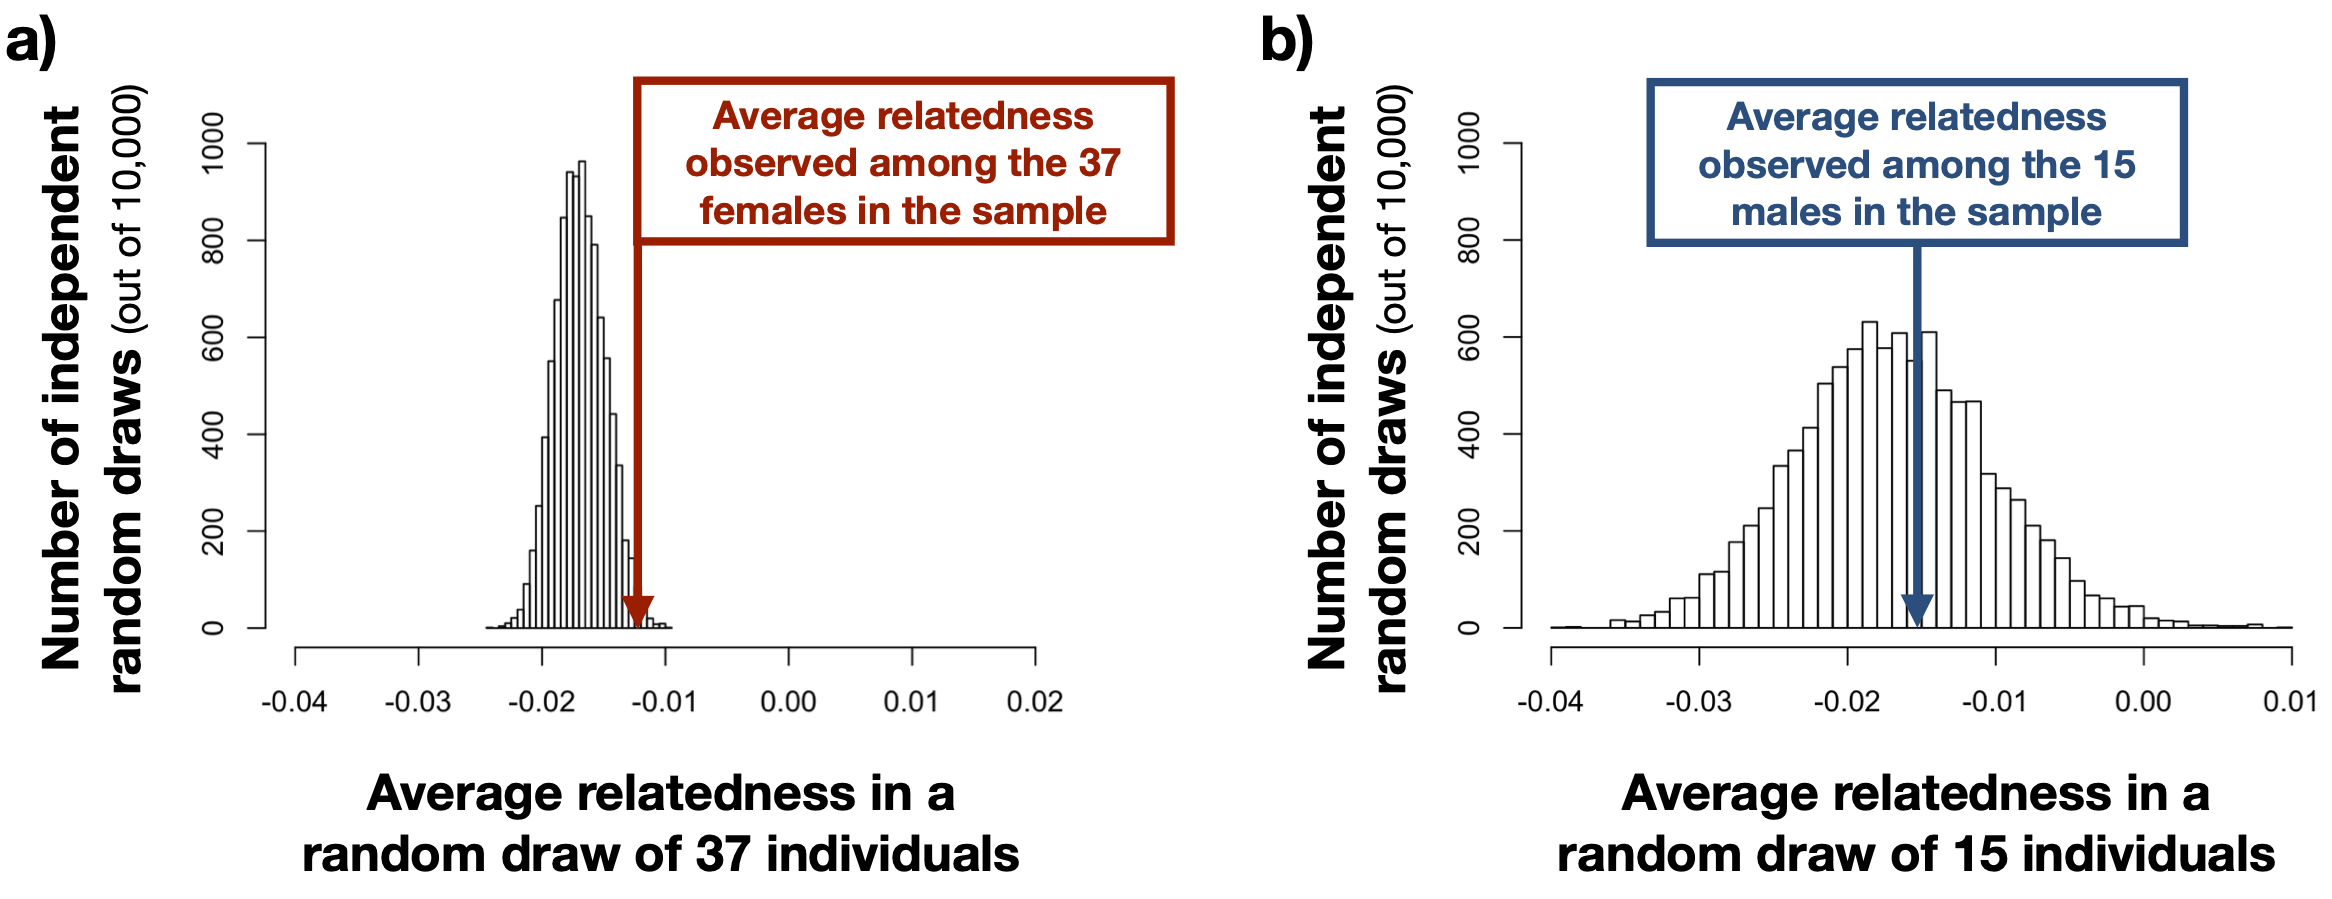
\includegraphics{gdispersal_Figure1.png}

\textbf{Figure 2.} Females are more related than expected by random
chance, whereas males are not. a) In less than 4\% of 10,000 repetitions
is the average relatedness among the 37 randomly drawn individuals (of
both sexes) as high as or higher than the observed relatedness among the
37 females in our sample. b) In contrast, average relatedness among 15
randomly drawn individuals (of both sexes) is higher than the observed
relatedness among the 15 males in our sample in 38\% of 10,000 draws.

\newpage

\hypertarget{analysis-ii-distances-among-genetic-relatives-1}{%
\paragraph{\texorpdfstring{\emph{Analysis ii: distances among genetic
relatives}}{Analysis ii: distances among genetic relatives}}\label{analysis-ii-distances-among-genetic-relatives-1}}

Close female genetic relatives are found to have been trapped in close
spatial proximity to each other (Figure 2). The median distance between
the eight female dyads related at 0.25 or higher is 340m (SD=440m) and
between the twelve female dyads related at 0.125 or higher is 360m
(SD=354m), compared to a median of 620m (SD=464m) among all dyads of
females (Figure 3). A median distance as short as or shorter than 340m
is observed in less than 6\% of all random samples of 7 female dyads and
a median distance of 360m or shorter is observed in less than 4\% of all
random samples of 12 female dyads. The distance among the one pair of
males related at higher than 0.25 is 670m, and the median distance among
the three male dyads related at 0.125 or higher is 1183m (SD=353m). This
compares to a median of 972m (SD=569m) among all dyads of males, with
about 40\% of male dyads being 670m or less apart. The difference in
distances among the 12 related females (r≥0.125, on average 360m apart)
compared to the three related males (r≥0.125, on average 1183m apart) is
823m. This difference in distance (and larger differences in distance)
is present in only 2\% of 10,000 random draws comparing average
distances among 12 random females and three random males.

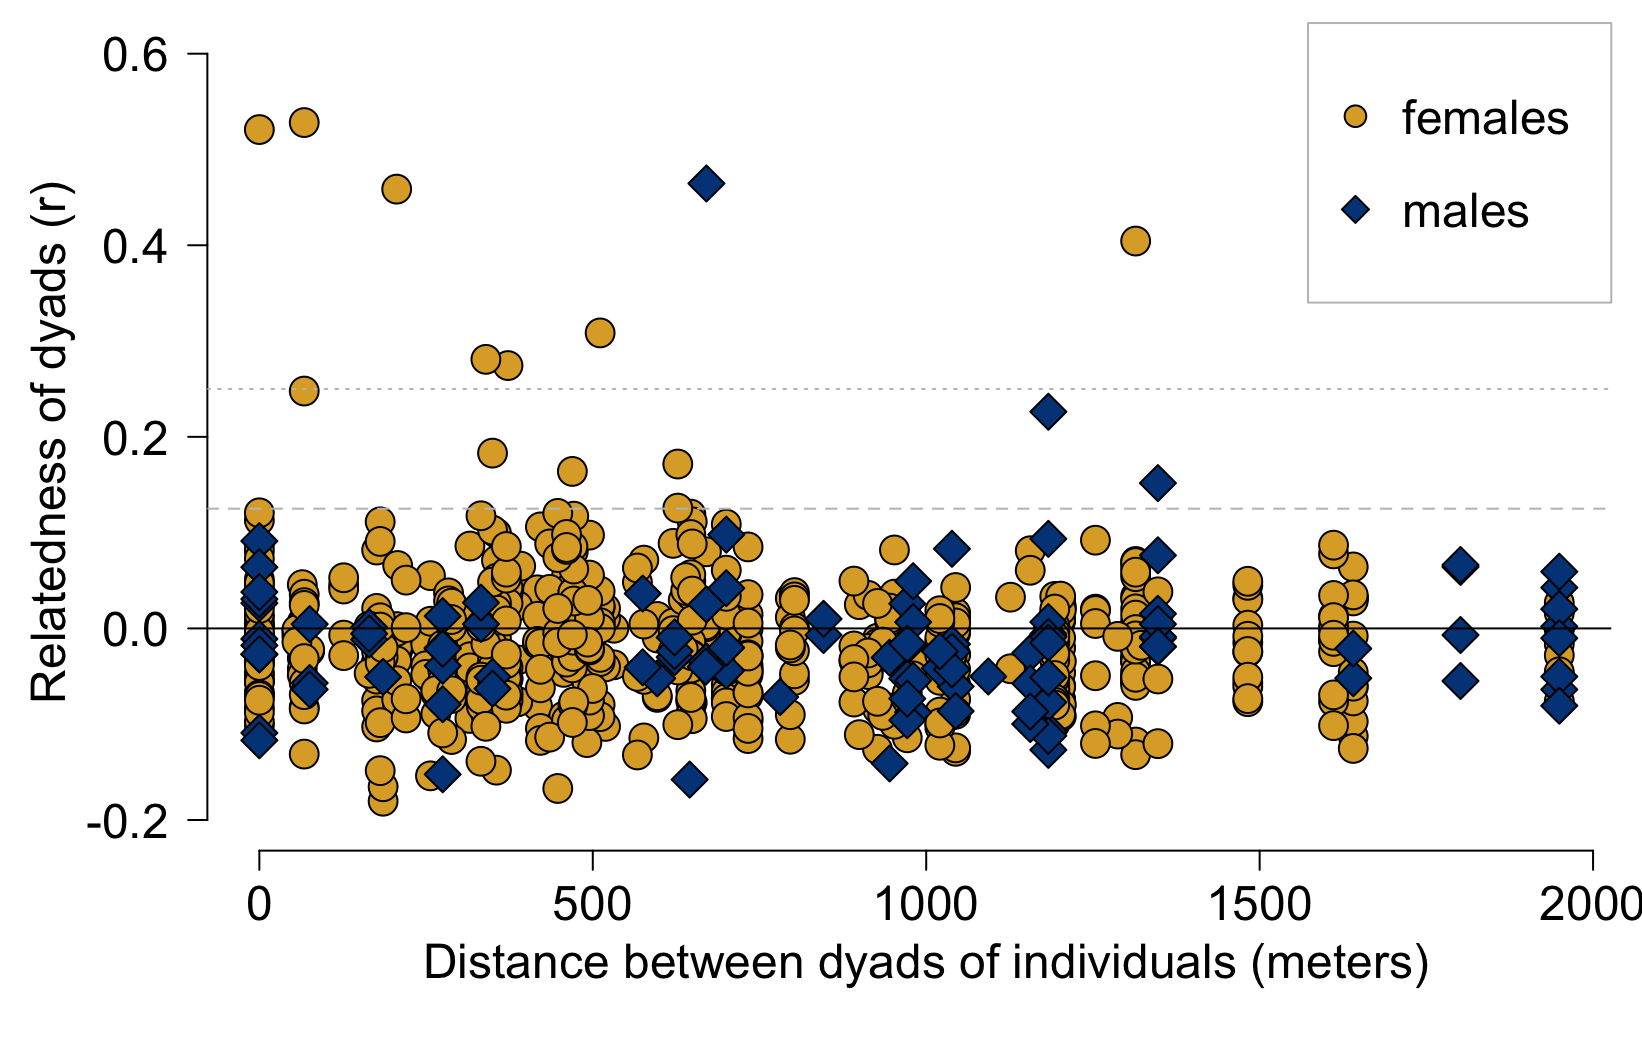
\includegraphics{gdispersal_Figure2.png}

\textbf{Figure 3.} Change in genetic relatedness as geographic distance
among dyads increases. Each dot reflects a single dyad, a pair of female
individuals (yellow) or a pair of male individuals (blue). There are
very few close male relatives who are found at larger distances. The
small number of close female relatives are all found within relatively
short distances of each other. The dotted horizontal line indicates the
level of relatedness for half-siblings (r=0.25), the dashed line
indicates the level of relatedness for cousins (r=0.125).

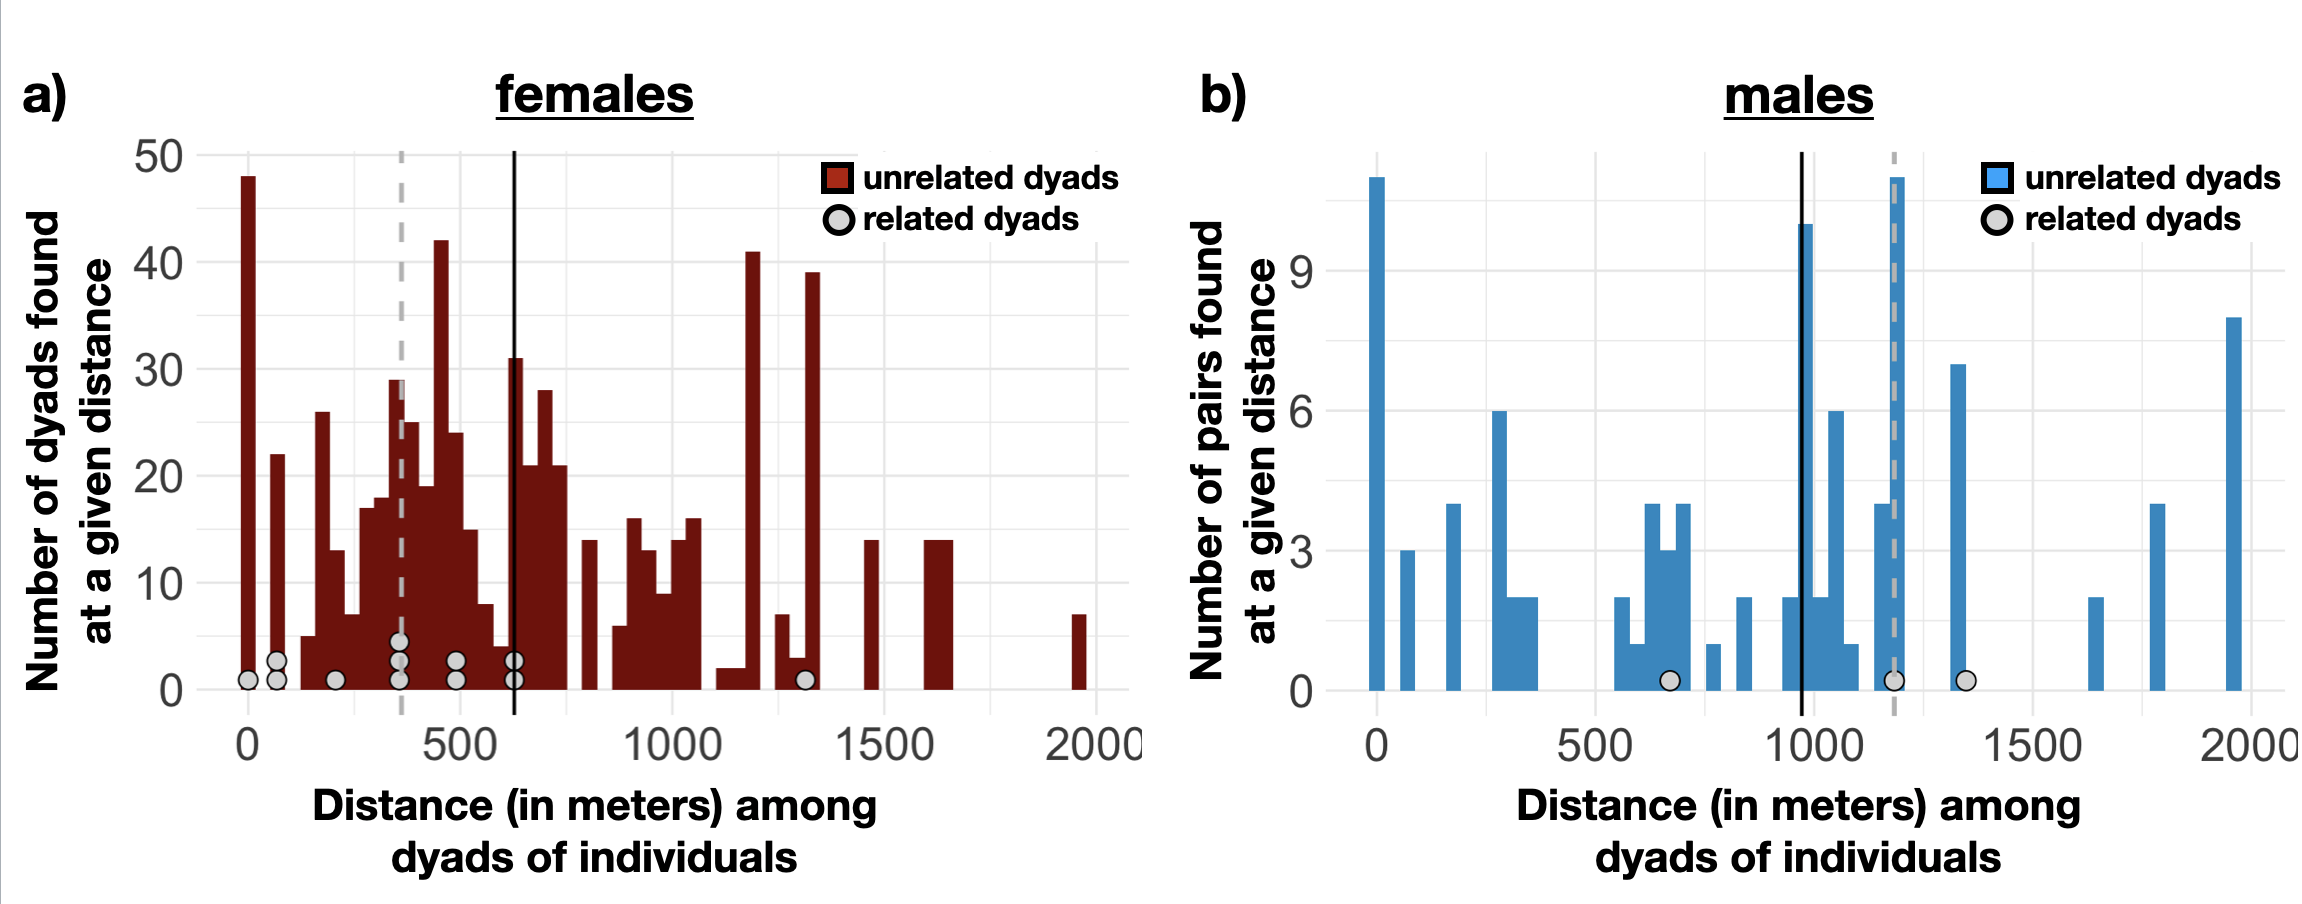
\includegraphics{gdispersal_Figure3.png}

\textbf{Figure 4.} The geographic distance among dyads of closely
related individuals (relatedness of 0.125 or higher; light circles)
compared to the distance among dyads of unrelated individuals (colored
bars). a) Among females, twelve closely related individuals were trapped
at locations near each other (median distance indicated by dotted grey
line), with eleven of the twelve closely related female dyads at
distances as near as or nearer than the median of unrelated female dyads
(vertical black line). b) In contrast, only one of the three closely
related male pairs was trapped at locations that were as near as or
nearer than the median distance among the unrelated males (vertical
black line). The distances among the closely related males were about
three times larger (median indicated by dotted grey line) than the
distances among closely related females.

\hypertarget{analysis-iii-spatial-autocorrelation-1}{%
\paragraph{\texorpdfstring{\emph{Analysis iii: spatial
autocorrelation}}{Analysis iii: spatial autocorrelation}}\label{analysis-iii-spatial-autocorrelation-1}}

Correlogram analyses linking genetic relatedness and spatial distance
for females showed negative values when females are in close spatial
proximity and positive values when they are far apart (the corrected
probability values for females are different than expected by chance in
two of the five distance classes), suggesting that as spatial distance
among females increases the relatedness among them decreases (Table 1).
Correlogram analyses for males showed no consistent relationships
between genetic relatedness and spatial distance, with values
fluctuating around zero (none of the corrected probability values for
males are different than expected by chance in any of the five distance
classes; Table 1).

\textbf{Table 1.} Output of correlogram analyses linking pairwise
relatedness to pairwise distances. The values represent the correlations
between relatedness and distances for males and females across trapping
sites binned into distance classes, with the probability of observing
the values by chance corrected for the multiple tests across distances
classes (based on the Holm-Bonferroni method).

\begin{longtable}[]{@{}lrrrr@{}}
\toprule
\begin{minipage}[b]{(\columnwidth - 4\tabcolsep) * \real{0.13}}\raggedright
Distance class\strut
\end{minipage} &
\begin{minipage}[b]{(\columnwidth - 4\tabcolsep) * \real{0.18}}\raggedleft
Females: correlation\strut
\end{minipage} &
\begin{minipage}[b]{(\columnwidth - 4\tabcolsep) * \real{0.27}}\raggedleft
Females: corrected probability\strut
\end{minipage} &
\begin{minipage}[b]{(\columnwidth - 4\tabcolsep) * \real{0.17}}\raggedleft
Males: correlation\strut
\end{minipage} &
\begin{minipage}[b]{(\columnwidth - 4\tabcolsep) * \real{0.25}}\raggedleft
Males: corrected probability\strut
\end{minipage}\tabularnewline
\midrule
\endhead
\begin{minipage}[t]{(\columnwidth - 4\tabcolsep) * \real{0.13}}\raggedright
0-150m\strut
\end{minipage} &
\begin{minipage}[t]{(\columnwidth - 4\tabcolsep) * \real{0.18}}\raggedleft
-0.10\strut
\end{minipage} &
\begin{minipage}[t]{(\columnwidth - 4\tabcolsep) * \real{0.27}}\raggedleft
0.01\strut
\end{minipage} &
\begin{minipage}[t]{(\columnwidth - 4\tabcolsep) * \real{0.17}}\raggedleft
-0.01\strut
\end{minipage} &
\begin{minipage}[t]{(\columnwidth - 4\tabcolsep) * \real{0.25}}\raggedleft
0.39\strut
\end{minipage}\tabularnewline
\begin{minipage}[t]{(\columnwidth - 4\tabcolsep) * \real{0.13}}\raggedright
150-450m\strut
\end{minipage} &
\begin{minipage}[t]{(\columnwidth - 4\tabcolsep) * \real{0.18}}\raggedleft
0.02\strut
\end{minipage} &
\begin{minipage}[t]{(\columnwidth - 4\tabcolsep) * \real{0.27}}\raggedleft
0.32\strut
\end{minipage} &
\begin{minipage}[t]{(\columnwidth - 4\tabcolsep) * \real{0.17}}\raggedleft
0.09\strut
\end{minipage} &
\begin{minipage}[t]{(\columnwidth - 4\tabcolsep) * \real{0.25}}\raggedleft
0.37\strut
\end{minipage}\tabularnewline
\begin{minipage}[t]{(\columnwidth - 4\tabcolsep) * \real{0.13}}\raggedright
450-900m\strut
\end{minipage} &
\begin{minipage}[t]{(\columnwidth - 4\tabcolsep) * \real{0.18}}\raggedleft
-0.05\strut
\end{minipage} &
\begin{minipage}[t]{(\columnwidth - 4\tabcolsep) * \real{0.27}}\raggedleft
0.25\strut
\end{minipage} &
\begin{minipage}[t]{(\columnwidth - 4\tabcolsep) * \real{0.17}}\raggedleft
-0.13\strut
\end{minipage} &
\begin{minipage}[t]{(\columnwidth - 4\tabcolsep) * \real{0.25}}\raggedleft
0.21\strut
\end{minipage}\tabularnewline
\begin{minipage}[t]{(\columnwidth - 4\tabcolsep) * \real{0.13}}\raggedright
900-1600m\strut
\end{minipage} &
\begin{minipage}[t]{(\columnwidth - 4\tabcolsep) * \real{0.18}}\raggedleft
0.10\strut
\end{minipage} &
\begin{minipage}[t]{(\columnwidth - 4\tabcolsep) * \real{0.27}}\raggedleft
0.04\strut
\end{minipage} &
\begin{minipage}[t]{(\columnwidth - 4\tabcolsep) * \real{0.17}}\raggedleft
0.09\strut
\end{minipage} &
\begin{minipage}[t]{(\columnwidth - 4\tabcolsep) * \real{0.25}}\raggedleft
0.55\strut
\end{minipage}\tabularnewline
\begin{minipage}[t]{(\columnwidth - 4\tabcolsep) * \real{0.13}}\raggedright
1600-2000m\strut
\end{minipage} &
\begin{minipage}[t]{(\columnwidth - 4\tabcolsep) * \real{0.18}}\raggedleft
0.01\strut
\end{minipage} &
\begin{minipage}[t]{(\columnwidth - 4\tabcolsep) * \real{0.27}}\raggedleft
0.66\strut
\end{minipage} &
\begin{minipage}[t]{(\columnwidth - 4\tabcolsep) * \real{0.17}}\raggedleft
-0.05\strut
\end{minipage} &
\begin{minipage}[t]{(\columnwidth - 4\tabcolsep) * \real{0.25}}\raggedleft
0.73\strut
\end{minipage}\tabularnewline
\bottomrule
\end{longtable}

\newpage

\hypertarget{discussion}{%
\subsection{Discussion}\label{discussion}}

Our results show that in great-tailed grackles, unlike in most other
bird species but in line with their divergent social and mating system,
the majority of males are not philopatric because individuals are not
found in close proximity to fathers or brothers. In contrast, several
female great-tailed grackles are found in close proximity to genetic
kin. The most likely explanation for this assortment of kin in space is
that at least some females remain close to where they hatched. Overall,
the findings support the first alternative hypothesis that males
disperse more than females. We find that the mean level of average
genetic relatedness is slightly lower among males compared to females in
our sample and that females are more closely related to each other than
expected by chance, while males are not (analysis i); the mean
geographic distance between pairs of individuals that are close genetic
relatives is higher among males compared to females (analysis ii); and
there is no spatial relationship between genetic relatedness and
geographic distance for males, while there is a negative spatial
autocorrelation signal indicating a negative relationship between
genetic relatedness and geographic distance for females (analysis iii).

Our small sample (we estimate that we trapped \textasciitilde25-30\% of
all grackles within this area, which is continuously connected to other
areas in which grackles reside) and the limited number of genetic
relatives we found, restrict the inferences we can draw. The consistency
of the results across the three types of analyses, showing that at least
some female great-tailed grackles remain close to relatives and most
males disperse, is reassuring and supports the inference that males
disperse more than females. Previous studies relying on spatial analyses
of multi-locus genotypes were also able to detect even modest sex biased
dispersal in fine-scale spatial distribution (examples of empirical
studies that detected a signal with small sample sizes include Hofmann
et al. 2012; Quaglietta et al. 2013; Gour et al. 2013; Botero-Delgadillo
et al. 2017). In particular, the effective number of SNP loci we have
for each individual likely increased our power to obtain a qualitative
assessment of whether relatives are present in our sample and,
accordingly, whether dispersal is more prevalent in females or males
based on spatial autocorrelation (Banks and Peakall 2012). However, we
cannot infer how substantial this sex bias is (our comparison of average
relatedness between sexes is inconclusive), what percentage of females
and males might disperse, or how far they might move. In addition,
because we only have information for a small number of individuals from
within a single site, we could not use methods that rely on assigning
individuals to a source population or measure the relative distribution
of genetic variation within versus among populations (Fst or similar
measures). Such approaches could reveal the proportion of individuals
who do disperse and the distances they might move, something which we
are planning to investigate in the future (see Logan et al. 2020).

Our findings indicate that great-tailed grackles are a species that
might help us better understand the factors influencing the dispersal
decisions of female and male birds. The reversal of the sex bias in
great-tailed grackles compared to what is observed in most other avian
species is in line with the main hypothesis that has been put forward to
explain the contrast in sex biases in dispersal between birds and
mammals: that in polygynous species, males disperse to search for mating
opportunities, while in monogamous species, males remain philopatric to
defend resources for high quality partners. However, given that the link
between the mating system and dispersal is more ambiguous than sometimes
assumed (Li and Kokko 2019) and given the limitations of our study, we
cannot determine the underlying reasons for why males disperse or why
females apparently remain close to where they hatched. We only observe a
general pattern of bias, but we do not have sufficiently detailed
information on the experiences of particular individuals that might have
shaped their dispersal behavior. Individual-based studies are needed to
investigate resource and mating competition and whether the patterning
of relatives in space relates to kin-based social interactions and
inbreeding. In addition, information on dispersal patterns from
different sites might help elucidate how much the sex bias we detect at
this site in the city center of Tempe is shaped by local factors or
whether it is linked to general features of the biology of great-tailed
grackles.

\newpage

\hypertarget{code}{%
\subsection{Code}\label{code}}

All data necessary for the analyses are available at
\url{https://doi.org/10.5063/F1W66J48} (Lukas 2020) and at github (the
provided code will load these files directly from github).

\hypertarget{load-data}{%
\paragraph{Load data}\label{load-data}}

\begin{Shaded}
\begin{Highlighting}[]
\FunctionTok{options}\NormalTok{(}\AttributeTok{width=}\DecValTok{60}\NormalTok{)}

\FunctionTok{library}\NormalTok{(related)}
\FunctionTok{library}\NormalTok{(tidyr)}
\FunctionTok{library}\NormalTok{(dplyr)}
\FunctionTok{library}\NormalTok{(vegan)}
\FunctionTok{library}\NormalTok{(geosphere)}
\FunctionTok{library}\NormalTok{(DataCombine)}
\FunctionTok{library}\NormalTok{(data.table)}
\FunctionTok{library}\NormalTok{(readr) }

\CommentTok{\#SNP data, processed to calculate pairwise relatedness}
\NormalTok{input}\OtherTok{\textless{}{-}}\FunctionTok{readgenotypedata}\NormalTok{(}\StringTok{"https://raw.githubusercontent.com/}
\StringTok{                        corinalogan/grackles/master/Files/Preregistrations/}
\StringTok{                        gDispersal\_GrackleGenotypesForRelatedness.txt"}\NormalTok{)}

\CommentTok{\# Individual level data, listing the sex (M ale or F emale), age (A dult or J uvenile), and latitude and longitude of the capture location}
\NormalTok{gracklelocations}\OtherTok{\textless{}{-}}\FunctionTok{read\_csv}\NormalTok{(}\FunctionTok{url}\NormalTok{(}\StringTok{"https://raw.githubusercontent.com/}
\StringTok{                              corinalogan/grackles/master/Files/Preregistrations/}
\StringTok{                              gDispersal\_GrackleIndividualInformationForRelatedness.csv"}\NormalTok{))}
\NormalTok{gracklelocations}\OtherTok{\textless{}{-}}\FunctionTok{data.frame}\NormalTok{(gracklelocations)}
\end{Highlighting}
\end{Shaded}

\hypertarget{subset-data-to-relevant-sample-excluding-juveniles-and-outlier-genotype}{%
\paragraph{Subset data to relevant sample, excluding juveniles and
outlier
genotype}\label{subset-data-to-relevant-sample-excluding-juveniles-and-outlier-genotype}}

\begin{Shaded}
\begin{Highlighting}[]
\FunctionTok{options}\NormalTok{(}\AttributeTok{width=}\DecValTok{60}\NormalTok{)}
\NormalTok{input}\SpecialCharTok{$}\NormalTok{gdata}\SpecialCharTok{$}\NormalTok{V1}\OtherTok{\textless{}{-}}\FunctionTok{as.character}\NormalTok{(gracklelocations}\SpecialCharTok{$}\NormalTok{Individual)}
\NormalTok{gracklelocations}\OtherTok{\textless{}{-}}\FunctionTok{filter}\NormalTok{(gracklelocations,Individual }\SpecialCharTok{!=} \StringTok{"AF\_053PS"}\NormalTok{)}
\NormalTok{adults}\OtherTok{\textless{}{-}}\FunctionTok{filter}\NormalTok{(gracklelocations,Age }\SpecialCharTok{\%in\%} \StringTok{"A"}\NormalTok{)[,]}\SpecialCharTok{$}\NormalTok{Individual}
\NormalTok{adultgracklelocations}\OtherTok{\textless{}{-}}\FunctionTok{filter}\NormalTok{(gracklelocations,Individual }\SpecialCharTok{\%in\%}\NormalTok{ adults)}
\end{Highlighting}
\end{Shaded}

\hypertarget{calculate-pairwise-distances-from-trapping-site-locations}{%
\paragraph{Calculate pairwise distances from trapping site
locations}\label{calculate-pairwise-distances-from-trapping-site-locations}}

\begin{Shaded}
\begin{Highlighting}[]
\FunctionTok{options}\NormalTok{(}\AttributeTok{width=}\DecValTok{60}\NormalTok{)}

\CommentTok{\#Plot pairwise distances among all females and among all males in the sample}
\CommentTok{\#Calculate all pairwise distances}
\NormalTok{all\_pairwise\_distances }\OtherTok{\textless{}{-}} \FunctionTok{distm}\NormalTok{(adultgracklelocations[,}\FunctionTok{c}\NormalTok{(}\StringTok{\textquotesingle{}Lon\textquotesingle{}}\NormalTok{,}\StringTok{\textquotesingle{}Lat\textquotesingle{}}\NormalTok{)], adultgracklelocations[,}\FunctionTok{c}\NormalTok{(}\StringTok{\textquotesingle{}Lon\textquotesingle{}}\NormalTok{,}\StringTok{\textquotesingle{}Lat\textquotesingle{}}\NormalTok{)], }\AttributeTok{fun=}\NormalTok{distVincentyEllipsoid)}
\FunctionTok{rownames}\NormalTok{(all\_pairwise\_distances)}\OtherTok{\textless{}{-}}\NormalTok{adultgracklelocations}\SpecialCharTok{$}\NormalTok{Individual}
\FunctionTok{colnames}\NormalTok{(all\_pairwise\_distances)}\OtherTok{\textless{}{-}}\NormalTok{adultgracklelocations}\SpecialCharTok{$}\NormalTok{Individual}
\FunctionTok{diag}\NormalTok{(all\_pairwise\_distances)}\OtherTok{\textless{}{-}}\ConstantTok{NA}

\CommentTok{\#Calculate pairwise distances among all the females}
\NormalTok{female\_pairwise\_distances }\OtherTok{\textless{}{-}} \FunctionTok{distm}\NormalTok{(adultgracklelocations[adultgracklelocations}\SpecialCharTok{$}\NormalTok{Sex}\SpecialCharTok{==}\StringTok{"F"}\NormalTok{,}\FunctionTok{c}\NormalTok{(}\StringTok{\textquotesingle{}Lon\textquotesingle{}}\NormalTok{,}\StringTok{\textquotesingle{}Lat\textquotesingle{}}\NormalTok{)], adultgracklelocations[adultgracklelocations}\SpecialCharTok{$}\NormalTok{Sex}\SpecialCharTok{==}\StringTok{"F"}\NormalTok{,}\FunctionTok{c}\NormalTok{(}\StringTok{\textquotesingle{}Lon\textquotesingle{}}\NormalTok{,}\StringTok{\textquotesingle{}Lat\textquotesingle{}}\NormalTok{)], }\AttributeTok{fun=}\NormalTok{distVincentyEllipsoid)}
\FunctionTok{rownames}\NormalTok{(female\_pairwise\_distances)}\OtherTok{\textless{}{-}}\NormalTok{adultgracklelocations[adultgracklelocations}\SpecialCharTok{$}\NormalTok{Sex}\SpecialCharTok{==}\StringTok{"F"}\NormalTok{,]}\SpecialCharTok{$}\NormalTok{Individual}
\FunctionTok{colnames}\NormalTok{(female\_pairwise\_distances)}\OtherTok{\textless{}{-}}\NormalTok{adultgracklelocations[adultgracklelocations}\SpecialCharTok{$}\NormalTok{Sex}\SpecialCharTok{==}\StringTok{"F"}\NormalTok{,]}\SpecialCharTok{$}\NormalTok{Individual}
\FunctionTok{diag}\NormalTok{(female\_pairwise\_distances)}\OtherTok{\textless{}{-}}\ConstantTok{NA}

\CommentTok{\#Calculate pairwise distances among all the females}
\NormalTok{male\_pairwise\_distances }\OtherTok{\textless{}{-}} \FunctionTok{distm}\NormalTok{(adultgracklelocations[adultgracklelocations}\SpecialCharTok{$}\NormalTok{Sex}\SpecialCharTok{==}\StringTok{"M"}\NormalTok{,}\FunctionTok{c}\NormalTok{(}\StringTok{\textquotesingle{}Lon\textquotesingle{}}\NormalTok{,}\StringTok{\textquotesingle{}Lat\textquotesingle{}}\NormalTok{)], adultgracklelocations[adultgracklelocations}\SpecialCharTok{$}\NormalTok{Sex}\SpecialCharTok{==}\StringTok{"M"}\NormalTok{,}\FunctionTok{c}\NormalTok{(}\StringTok{\textquotesingle{}Lon\textquotesingle{}}\NormalTok{,}\StringTok{\textquotesingle{}Lat\textquotesingle{}}\NormalTok{)], }\AttributeTok{fun=}\NormalTok{distVincentyEllipsoid)}
\FunctionTok{rownames}\NormalTok{(male\_pairwise\_distances)}\OtherTok{\textless{}{-}}\NormalTok{adultgracklelocations[adultgracklelocations}\SpecialCharTok{$}\NormalTok{Sex}\SpecialCharTok{==}\StringTok{"M"}\NormalTok{,]}\SpecialCharTok{$}\NormalTok{Individual}
\FunctionTok{colnames}\NormalTok{(male\_pairwise\_distances)}\OtherTok{\textless{}{-}}\NormalTok{adultgracklelocations[adultgracklelocations}\SpecialCharTok{$}\NormalTok{Sex}\SpecialCharTok{==}\StringTok{"M"}\NormalTok{,]}\SpecialCharTok{$}\NormalTok{Individual}
\FunctionTok{diag}\NormalTok{(male\_pairwise\_distances)}\OtherTok{\textless{}{-}}\ConstantTok{NA}

\CommentTok{\#plot distributions of pairwise distances}
\FunctionTok{hist}\NormalTok{(all\_pairwise\_distances,}\AttributeTok{col=}\StringTok{"grey75"}\NormalTok{,}\AttributeTok{border=}\StringTok{"black"}\NormalTok{,}\AttributeTok{breaks=}\DecValTok{10}\NormalTok{)}
\FunctionTok{hist}\NormalTok{(female\_pairwise\_distances,}\AttributeTok{col=}\StringTok{"grey75"}\NormalTok{,}\AttributeTok{border=}\StringTok{"black"}\NormalTok{,}\AttributeTok{breaks=}\DecValTok{10}\NormalTok{)}
\FunctionTok{hist}\NormalTok{(male\_pairwise\_distances,}\AttributeTok{col=}\StringTok{"grey75"}\NormalTok{,}\AttributeTok{border=}\StringTok{"black"}\NormalTok{,}\AttributeTok{breaks=}\DecValTok{10}\NormalTok{)}
\end{Highlighting}
\end{Shaded}

\hypertarget{analysis-i-average-relatedness-and-sex-2}{%
\paragraph{\texorpdfstring{\emph{Analysis i: average relatedness and
sex}}{Analysis i: average relatedness and sex}}\label{analysis-i-average-relatedness-and-sex-2}}

\begin{Shaded}
\begin{Highlighting}[]
\FunctionTok{options}\NormalTok{(}\AttributeTok{width=}\DecValTok{60}\NormalTok{)}

\CommentTok{\#Analysis 1: Assess whether average relatedness is higher among females or among males}
\CommentTok{\#Calculate pairwise relatedness, here choosing the relatedness method developed by Wang and Queller \& Goodnight}
\NormalTok{outfile}\OtherTok{\textless{}{-}}\FunctionTok{coancestry}\NormalTok{(input}\SpecialCharTok{$}\NormalTok{gdata,}\AttributeTok{wang=}\DecValTok{1}\NormalTok{,}\AttributeTok{quellergt=}\DecValTok{1}\NormalTok{)}

\CommentTok{\#extract the relevant information from the file}
\NormalTok{pairwise\_r}\OtherTok{\textless{}{-}}\NormalTok{outfile}\SpecialCharTok{$}\NormalTok{relatedness}

\CommentTok{\# We now exclude the individual with the dubious genotype and the juvenile individuals}
\NormalTok{pairwise\_r}\OtherTok{\textless{}{-}}\FunctionTok{filter}\NormalTok{(pairwise\_r,ind1.id }\SpecialCharTok{!=} \StringTok{"AF\_053PS"}\NormalTok{)}
\NormalTok{pairwise\_r}\OtherTok{\textless{}{-}}\FunctionTok{filter}\NormalTok{(pairwise\_r,ind2.id }\SpecialCharTok{!=} \StringTok{"AF\_053PS"}\NormalTok{)}

\CommentTok{\# Next, we exculde all juvenile individuals}
\NormalTok{pairwise\_r}\OtherTok{\textless{}{-}}\FunctionTok{filter}\NormalTok{(pairwise\_r,ind1.id }\SpecialCharTok{\%in\%}\NormalTok{ adults)}
\NormalTok{pairwise\_r}\OtherTok{\textless{}{-}}\FunctionTok{filter}\NormalTok{(pairwise\_r,ind2.id }\SpecialCharTok{\%in\%}\NormalTok{ adults)}

\CommentTok{\#This leaves us with 1326 pairwise relatedness values among the 52 remaining individuals}


\CommentTok{\#identify which individuals are female and which are male}
\NormalTok{females}\OtherTok{\textless{}{-}}\FunctionTok{filter}\NormalTok{(gracklelocations,Sex }\SpecialCharTok{\%in\%} \StringTok{"F"}\NormalTok{,Age }\SpecialCharTok{\%in\%} \StringTok{"A"}\NormalTok{)[,]}\SpecialCharTok{$}\NormalTok{Individual}
\NormalTok{males}\OtherTok{\textless{}{-}}\FunctionTok{filter}\NormalTok{(gracklelocations,Sex }\SpecialCharTok{\%in\%} \StringTok{"M"}\NormalTok{,Age }\SpecialCharTok{\%in\%} \StringTok{"A"}\NormalTok{)[,]}\SpecialCharTok{$}\NormalTok{Individual}

\CommentTok{\#Calculate average of and variance in relatedness among all individuals, all females, and all males}
\CommentTok{\# First using the relatedness estimates based on the method by Wang}
\FunctionTok{mean}\NormalTok{(}\FunctionTok{filter}\NormalTok{(pairwise\_r,ind1.id }\SpecialCharTok{\%in\%}\NormalTok{ females,ind2.id }\SpecialCharTok{\%in\%}\NormalTok{ females)}\SpecialCharTok{$}\NormalTok{wang)}
\FunctionTok{mean}\NormalTok{(}\FunctionTok{filter}\NormalTok{(pairwise\_r,ind1.id }\SpecialCharTok{\%in\%}\NormalTok{ males,ind2.id }\SpecialCharTok{\%in\%}\NormalTok{ males)}\SpecialCharTok{$}\NormalTok{wang)}
\FunctionTok{mean}\NormalTok{(pairwise\_r}\SpecialCharTok{$}\NormalTok{wang)}

\FunctionTok{var}\NormalTok{(}\FunctionTok{filter}\NormalTok{(pairwise\_r,ind1.id }\SpecialCharTok{\%in\%}\NormalTok{ females,ind2.id }\SpecialCharTok{\%in\%}\NormalTok{ females)}\SpecialCharTok{$}\NormalTok{wang)}
\FunctionTok{var}\NormalTok{(}\FunctionTok{filter}\NormalTok{(pairwise\_r,ind1.id }\SpecialCharTok{\%in\%}\NormalTok{ males,ind2.id }\SpecialCharTok{\%in\%}\NormalTok{ males)}\SpecialCharTok{$}\NormalTok{wang)}
\FunctionTok{var}\NormalTok{(pairwise\_r}\SpecialCharTok{$}\NormalTok{wang)}

\CommentTok{\# Next using the relatedness estimates based on the method by Queller and Goodnight}
\FunctionTok{mean}\NormalTok{(}\FunctionTok{filter}\NormalTok{(pairwise\_r,ind1.id }\SpecialCharTok{\%in\%}\NormalTok{ females,ind2.id }\SpecialCharTok{\%in\%}\NormalTok{ females)}\SpecialCharTok{$}\NormalTok{quellergt)}
\FunctionTok{mean}\NormalTok{(}\FunctionTok{filter}\NormalTok{(pairwise\_r,ind1.id }\SpecialCharTok{\%in\%}\NormalTok{ males,ind2.id }\SpecialCharTok{\%in\%}\NormalTok{ males)}\SpecialCharTok{$}\NormalTok{quellergt)}
\FunctionTok{mean}\NormalTok{(pairwise\_r}\SpecialCharTok{$}\NormalTok{quellergt)}

\FunctionTok{var}\NormalTok{(}\FunctionTok{filter}\NormalTok{(pairwise\_r,ind1.id }\SpecialCharTok{\%in\%}\NormalTok{ females,ind2.id }\SpecialCharTok{\%in\%}\NormalTok{ females)}\SpecialCharTok{$}\NormalTok{quellergt)}
\FunctionTok{var}\NormalTok{(}\FunctionTok{filter}\NormalTok{(pairwise\_r,ind1.id }\SpecialCharTok{\%in\%}\NormalTok{ males,ind2.id }\SpecialCharTok{\%in\%}\NormalTok{ males)}\SpecialCharTok{$}\NormalTok{quellergt)}
\FunctionTok{var}\NormalTok{(pairwise\_r}\SpecialCharTok{$}\NormalTok{quellergt)}


\CommentTok{\#Perform a simulation to assess whether average relatedness among males is different from what we would expect in a random subset of the same number of individuals}
\CommentTok{\#First based on the relatedness estimates based on the method by Wang}
\NormalTok{simulatedrelatedness}\OtherTok{\textless{}{-}}\FunctionTok{matrix}\NormalTok{(}\AttributeTok{ncol=}\DecValTok{1}\NormalTok{,}\AttributeTok{nrow=}\DecValTok{10000}\NormalTok{)}
\ControlFlowTok{for}\NormalTok{ (i }\ControlFlowTok{in} \DecValTok{1}\SpecialCharTok{:}\DecValTok{10000}\NormalTok{) \{}
\NormalTok{  currentset}\OtherTok{\textless{}{-}}\FunctionTok{sample}\NormalTok{(adults,}\FunctionTok{length}\NormalTok{(males))}
\NormalTok{  simulatedrelatedness[i,}\DecValTok{1}\NormalTok{]}\OtherTok{\textless{}{-}}\FunctionTok{mean}\NormalTok{(}\FunctionTok{filter}\NormalTok{(pairwise\_r,ind1.id }\SpecialCharTok{\%in\%}\NormalTok{ currentset,ind2.id }\SpecialCharTok{\%in\%}\NormalTok{ currentset)}\SpecialCharTok{$}\NormalTok{wang)}
\NormalTok{\}}
\FunctionTok{hist}\NormalTok{(simulatedrelatedness)}
\CommentTok{\#This value is similar to a p{-}value, it reflects the probability that the average relatedness observed among males would be expected in a random subsample}
\FunctionTok{sum}\NormalTok{(simulatedrelatedness}\SpecialCharTok{\textgreater{}}\FunctionTok{mean}\NormalTok{(}\FunctionTok{filter}\NormalTok{(pairwise\_r,ind1.id }\SpecialCharTok{\%in\%}\NormalTok{ males,ind2.id }\SpecialCharTok{\%in\%}\NormalTok{ males)}\SpecialCharTok{$}\NormalTok{wang))}\SpecialCharTok{/}\DecValTok{10000}


\CommentTok{\#Perform a simulation to assess whether average relatedness among females is different from what we would expect in a random subset of the same number of individuals}
\NormalTok{simulatedrelatedness}\OtherTok{\textless{}{-}}\FunctionTok{matrix}\NormalTok{(}\AttributeTok{ncol=}\DecValTok{1}\NormalTok{,}\AttributeTok{nrow=}\DecValTok{10000}\NormalTok{)}
\ControlFlowTok{for}\NormalTok{ (i }\ControlFlowTok{in} \DecValTok{1}\SpecialCharTok{:}\DecValTok{10000}\NormalTok{) \{}
\NormalTok{  currentset}\OtherTok{\textless{}{-}}\FunctionTok{sample}\NormalTok{(adults,}\FunctionTok{length}\NormalTok{(females))}
\NormalTok{  simulatedrelatedness[i,}\DecValTok{1}\NormalTok{]}\OtherTok{\textless{}{-}}\FunctionTok{mean}\NormalTok{(}\FunctionTok{filter}\NormalTok{(pairwise\_r,ind1.id }\SpecialCharTok{\%in\%}\NormalTok{ currentset,ind2.id }\SpecialCharTok{\%in\%}\NormalTok{ currentset)}\SpecialCharTok{$}\NormalTok{wang)}
\NormalTok{\}}
\FunctionTok{hist}\NormalTok{(simulatedrelatedness)}
\CommentTok{\#This value is similar to a p{-}value, it reflects the probability that the average relatedness observed among males would be expected in a random subsample}
\FunctionTok{sum}\NormalTok{(simulatedrelatedness}\SpecialCharTok{\textgreater{}}\FunctionTok{mean}\NormalTok{(}\FunctionTok{filter}\NormalTok{(pairwise\_r,ind1.id }\SpecialCharTok{\%in\%}\NormalTok{ females,ind2.id }\SpecialCharTok{\%in\%}\NormalTok{ females)}\SpecialCharTok{$}\NormalTok{wang))}\SpecialCharTok{/}\DecValTok{10000}


\CommentTok{\#Next based on the relatedness estimates based on the method by Queller \& Goodnight}
\CommentTok{\#Perform a simulation to assess whether average relatedness among males is different from what we would expect in a random subset of the same number of individuals}
\NormalTok{simulatedrelatedness}\OtherTok{\textless{}{-}}\FunctionTok{matrix}\NormalTok{(}\AttributeTok{ncol=}\DecValTok{1}\NormalTok{,}\AttributeTok{nrow=}\DecValTok{10000}\NormalTok{)}
\ControlFlowTok{for}\NormalTok{ (i }\ControlFlowTok{in} \DecValTok{1}\SpecialCharTok{:}\DecValTok{10000}\NormalTok{) \{}
\NormalTok{  currentset}\OtherTok{\textless{}{-}}\FunctionTok{sample}\NormalTok{(adults,}\FunctionTok{length}\NormalTok{(males))}
\NormalTok{  simulatedrelatedness[i,}\DecValTok{1}\NormalTok{]}\OtherTok{\textless{}{-}}\FunctionTok{mean}\NormalTok{(}\FunctionTok{filter}\NormalTok{(pairwise\_r,ind1.id }\SpecialCharTok{\%in\%}\NormalTok{ currentset,ind2.id }\SpecialCharTok{\%in\%}\NormalTok{ currentset)}\SpecialCharTok{$}\NormalTok{quellergt)}
\NormalTok{\}}
\FunctionTok{hist}\NormalTok{(simulatedrelatedness)}
\CommentTok{\#This value is similar to a p{-}value, it reflects the probability that the average relatedness observed among males would be expected in a random subsample}
\FunctionTok{sum}\NormalTok{(simulatedrelatedness}\SpecialCharTok{\textgreater{}}\FunctionTok{mean}\NormalTok{(}\FunctionTok{filter}\NormalTok{(pairwise\_r,ind1.id }\SpecialCharTok{\%in\%}\NormalTok{ males,ind2.id }\SpecialCharTok{\%in\%}\NormalTok{ males)}\SpecialCharTok{$}\NormalTok{quellergt))}\SpecialCharTok{/}\DecValTok{10000}


\CommentTok{\#Perform a simulation to assess whether average relatedness among females is different from what we would expect in a random subset of the same number of individuals}
\NormalTok{simulatedrelatedness}\OtherTok{\textless{}{-}}\FunctionTok{matrix}\NormalTok{(}\AttributeTok{ncol=}\DecValTok{1}\NormalTok{,}\AttributeTok{nrow=}\DecValTok{10000}\NormalTok{)}
\ControlFlowTok{for}\NormalTok{ (i }\ControlFlowTok{in} \DecValTok{1}\SpecialCharTok{:}\DecValTok{10000}\NormalTok{) \{}
\NormalTok{  currentset}\OtherTok{\textless{}{-}}\FunctionTok{sample}\NormalTok{(adults,}\FunctionTok{length}\NormalTok{(females))}
\NormalTok{  simulatedrelatedness[i,}\DecValTok{1}\NormalTok{]}\OtherTok{\textless{}{-}}\FunctionTok{mean}\NormalTok{(}\FunctionTok{filter}\NormalTok{(pairwise\_r,ind1.id }\SpecialCharTok{\%in\%}\NormalTok{ currentset,ind2.id }\SpecialCharTok{\%in\%}\NormalTok{ currentset)}\SpecialCharTok{$}\NormalTok{quellergt)}
\NormalTok{\}}
\FunctionTok{hist}\NormalTok{(simulatedrelatedness)}
\CommentTok{\#This value is similar to a p{-}value, it reflects the probability that the average relatedness observed among males would be expected in a random subsample}
\FunctionTok{sum}\NormalTok{(simulatedrelatedness}\SpecialCharTok{\textgreater{}}\FunctionTok{mean}\NormalTok{(}\FunctionTok{filter}\NormalTok{(pairwise\_r,ind1.id }\SpecialCharTok{\%in\%}\NormalTok{ females,ind2.id }\SpecialCharTok{\%in\%}\NormalTok{ females)}\SpecialCharTok{$}\NormalTok{quellergt))}\SpecialCharTok{/}\DecValTok{10000}
\end{Highlighting}
\end{Shaded}

\hypertarget{analysis-ii-distances-among-genetic-relatives-2}{%
\paragraph{\texorpdfstring{\emph{Analysis ii: distances among genetic
relatives}}{Analysis ii: distances among genetic relatives}}\label{analysis-ii-distances-among-genetic-relatives-2}}

\begin{Shaded}
\begin{Highlighting}[]
\FunctionTok{options}\NormalTok{(}\AttributeTok{width=}\DecValTok{60}\NormalTok{)}

\CommentTok{\#Analysis 2: Assess whether distances among closely related females are shorter than distances among closely related males}
\CommentTok{\#First define close relatives as all pairs of individuals who are related by a level of 0.25 or higher (half{-}siblings or higher) using the Wang estimator}
\NormalTok{close\_relatives\_females}\OtherTok{\textless{}{-}}\FunctionTok{filter}\NormalTok{(pairwise\_r,wang }\SpecialCharTok{\textgreater{}}\FloatTok{0.2499}\NormalTok{,ind1.id }\SpecialCharTok{\%in\%}\NormalTok{ females,ind2.id }\SpecialCharTok{\%in\%}\NormalTok{ females)}
\NormalTok{close\_relatives\_females\_individuals}\OtherTok{\textless{}{-}}\FunctionTok{c}\NormalTok{(close\_relatives\_females}\SpecialCharTok{$}\NormalTok{ind1.id,close\_relatives\_females}\SpecialCharTok{$}\NormalTok{ind2.id)}

\CommentTok{\#Alternatively, select close relatives as pairs of individuals who are related at a level of 0.25 of higher using the Queller \& Goodnight estimator}
\NormalTok{close\_relatives\_females}\OtherTok{\textless{}{-}}\FunctionTok{filter}\NormalTok{(pairwise\_r,quellergt }\SpecialCharTok{\textgreater{}}\FloatTok{0.2499}\NormalTok{,ind1.id }\SpecialCharTok{\%in\%}\NormalTok{ females,ind2.id }\SpecialCharTok{\%in\%}\NormalTok{ females)}
\NormalTok{close\_relatives\_females\_individuals}\OtherTok{\textless{}{-}}\FunctionTok{c}\NormalTok{(close\_relatives\_females}\SpecialCharTok{$}\NormalTok{ind1.id,close\_relatives\_females}\SpecialCharTok{$}\NormalTok{ind2.id)}

\CommentTok{\#Pick one of the two estimators before proceeding with the following analyses}

\CommentTok{\#Next subset the the distance matrix to only include these individuals}

\NormalTok{females\_pairwise\_distances\_matrix}\OtherTok{\textless{}{-}}\FunctionTok{as.data.frame}\NormalTok{(female\_pairwise\_distances)}
\NormalTok{close\_relatives\_females\_pairwise\_distances}\OtherTok{\textless{}{-}}\FunctionTok{matrix}\NormalTok{(}\AttributeTok{nrow=}\FunctionTok{nrow}\NormalTok{(close\_relatives\_females),}\AttributeTok{ncol=}\DecValTok{1}\NormalTok{)}

\ControlFlowTok{for}\NormalTok{ (i }\ControlFlowTok{in} \DecValTok{1}\SpecialCharTok{:}\FunctionTok{nrow}\NormalTok{(close\_relatives\_females)) \{}
\NormalTok{  ind1}\OtherTok{\textless{}{-}}\NormalTok{close\_relatives\_females[i,]}\SpecialCharTok{$}\NormalTok{ind1.id}
\NormalTok{  ind2}\OtherTok{\textless{}{-}}\NormalTok{close\_relatives\_females[i,]}\SpecialCharTok{$}\NormalTok{ind2.id}
\NormalTok{  pair\_distance}\OtherTok{\textless{}{-}}\NormalTok{females\_pairwise\_distances\_matrix[ind1,ind2]}
\NormalTok{  close\_relatives\_females\_pairwise\_distances[i,]}\OtherTok{\textless{}{-}}\NormalTok{pair\_distance}
\NormalTok{\}}

\FunctionTok{median}\NormalTok{(close\_relatives\_females\_pairwise\_distances)}

\FunctionTok{hist}\NormalTok{(close\_relatives\_females\_pairwise\_distances)}


\CommentTok{\#repeat the same for the males}
\NormalTok{close\_relatives\_males}\OtherTok{\textless{}{-}}\FunctionTok{filter}\NormalTok{(pairwise\_r,wang }\SpecialCharTok{\textgreater{}}\FloatTok{0.2499}\NormalTok{,ind1.id }\SpecialCharTok{\%in\%}\NormalTok{ males,ind2.id }\SpecialCharTok{\%in\%}\NormalTok{ males)}
\NormalTok{close\_relatives\_males\_individuals}\OtherTok{\textless{}{-}}\FunctionTok{c}\NormalTok{(close\_relatives\_males}\SpecialCharTok{$}\NormalTok{ind1.id,close\_relatives\_males}\SpecialCharTok{$}\NormalTok{ind2.id)}

\CommentTok{\#Again, the alternative with the Queller \& Goodnight method, pick only one of the two}
\NormalTok{close\_relatives\_males}\OtherTok{\textless{}{-}}\FunctionTok{filter}\NormalTok{(pairwise\_r,quellergt }\SpecialCharTok{\textgreater{}}\FloatTok{0.2499}\NormalTok{,ind1.id }\SpecialCharTok{\%in\%}\NormalTok{ males,ind2.id }\SpecialCharTok{\%in\%}\NormalTok{ males)}
\NormalTok{close\_relatives\_males\_individuals}\OtherTok{\textless{}{-}}\FunctionTok{c}\NormalTok{(close\_relatives\_males}\SpecialCharTok{$}\NormalTok{ind1.id,close\_relatives\_males}\SpecialCharTok{$}\NormalTok{ind2.id)}


\CommentTok{\#Next subset the the distance matrix to only include these individuals}

\NormalTok{males\_pairwise\_distances\_matrix}\OtherTok{\textless{}{-}}\FunctionTok{as.data.frame}\NormalTok{(male\_pairwise\_distances)}
\NormalTok{close\_relatives\_males\_pairwise\_distances}\OtherTok{\textless{}{-}}\FunctionTok{matrix}\NormalTok{(}\AttributeTok{nrow=}\FunctionTok{nrow}\NormalTok{(close\_relatives\_males),}\AttributeTok{ncol=}\DecValTok{1}\NormalTok{)}

\ControlFlowTok{for}\NormalTok{ (i }\ControlFlowTok{in} \DecValTok{1}\SpecialCharTok{:}\FunctionTok{nrow}\NormalTok{(close\_relatives\_males)) \{}
\NormalTok{  ind1}\OtherTok{\textless{}{-}}\NormalTok{close\_relatives\_males[i,]}\SpecialCharTok{$}\NormalTok{ind1.id}
\NormalTok{  ind2}\OtherTok{\textless{}{-}}\NormalTok{close\_relatives\_males[i,]}\SpecialCharTok{$}\NormalTok{ind2.id}
\NormalTok{  pair\_distance}\OtherTok{\textless{}{-}}\NormalTok{males\_pairwise\_distances\_matrix[ind1,ind2]}
\NormalTok{  close\_relatives\_males\_pairwise\_distances[i,]}\OtherTok{\textless{}{-}}\NormalTok{pair\_distance}
\NormalTok{\}}

\FunctionTok{median}\NormalTok{(close\_relatives\_males\_pairwise\_distances)}

\FunctionTok{hist}\NormalTok{(close\_relatives\_males\_pairwise\_distances)}

\CommentTok{\#calculate difference between the distances among males and among females}
\NormalTok{observeddifferenceindistances}\OtherTok{\textless{}{-}}\FunctionTok{median}\NormalTok{(close\_relatives\_males\_pairwise\_distances,}\AttributeTok{na.rm=}\NormalTok{T)}\SpecialCharTok{{-}}\FunctionTok{median}\NormalTok{(close\_relatives\_females\_pairwise\_distances,}\AttributeTok{na.rm=}\NormalTok{T)}

\CommentTok{\#perform simulation to generate random draws of matching numbers of individuals to assess whether the sex{-}difference in the distance is more or less than what would be expected by chance}
\NormalTok{number\_close\_relatives\_females}\OtherTok{\textless{}{-}}\FunctionTok{nrow}\NormalTok{(close\_relatives\_females)}
\NormalTok{number\_close\_relatives\_males}\OtherTok{\textless{}{-}}\FunctionTok{nrow}\NormalTok{(close\_relatives\_males)}

\NormalTok{simulateddifferencesindistances}\OtherTok{\textless{}{-}}\FunctionTok{matrix}\NormalTok{(}\AttributeTok{ncol=}\DecValTok{1}\NormalTok{,}\AttributeTok{nrow=}\DecValTok{10000}\NormalTok{)}
\NormalTok{simulateddfemaleindistances}\OtherTok{\textless{}{-}}\FunctionTok{matrix}\NormalTok{(}\AttributeTok{ncol=}\DecValTok{1}\NormalTok{,}\AttributeTok{nrow=}\DecValTok{10000}\NormalTok{)}
\NormalTok{simulateddmaleindistances}\OtherTok{\textless{}{-}}\FunctionTok{matrix}\NormalTok{(}\AttributeTok{ncol=}\DecValTok{1}\NormalTok{,}\AttributeTok{nrow=}\DecValTok{10000}\NormalTok{)}

\ControlFlowTok{for}\NormalTok{ (i }\ControlFlowTok{in} \DecValTok{1}\SpecialCharTok{:}\DecValTok{10000}\NormalTok{) \{}
\NormalTok{simulated\_close\_relatives\_females}\OtherTok{\textless{}{-}}\FunctionTok{sample\_n}\NormalTok{(pairwise\_r, number\_close\_relatives\_females, }\AttributeTok{replace =} \ConstantTok{TRUE}\NormalTok{)}

\NormalTok{subset\_relatives\_females\_pairwise\_distances}\OtherTok{\textless{}{-}}\FunctionTok{matrix}\NormalTok{(}\AttributeTok{nrow=}\FunctionTok{nrow}\NormalTok{(simulated\_close\_relatives\_females),}\AttributeTok{ncol=}\DecValTok{1}\NormalTok{)}

\ControlFlowTok{for}\NormalTok{ (j }\ControlFlowTok{in} \DecValTok{1}\SpecialCharTok{:}\FunctionTok{nrow}\NormalTok{(simulated\_close\_relatives\_females)) \{}
\NormalTok{  ind1}\OtherTok{\textless{}{-}}\NormalTok{simulated\_close\_relatives\_females[j,]}\SpecialCharTok{$}\NormalTok{ind1.id}
\NormalTok{  ind2}\OtherTok{\textless{}{-}}\NormalTok{simulated\_close\_relatives\_females[j,]}\SpecialCharTok{$}\NormalTok{ind2.id}
\NormalTok{  pair\_distance}\OtherTok{\textless{}{-}}\NormalTok{all\_pairwise\_distances[ind1,ind2]}
\NormalTok{  subset\_relatives\_females\_pairwise\_distances[j,]}\OtherTok{\textless{}{-}}\NormalTok{pair\_distance}
\NormalTok{\}}

\NormalTok{simulated\_close\_relatives\_males}\OtherTok{\textless{}{-}}\FunctionTok{sample\_n}\NormalTok{(pairwise\_r, number\_close\_relatives\_males, }\AttributeTok{replace =} \ConstantTok{TRUE}\NormalTok{)}

\NormalTok{subset\_relatives\_males\_pairwise\_distances}\OtherTok{\textless{}{-}}\FunctionTok{matrix}\NormalTok{(}\AttributeTok{nrow=}\FunctionTok{nrow}\NormalTok{(simulated\_close\_relatives\_males),}\AttributeTok{ncol=}\DecValTok{1}\NormalTok{)}

\ControlFlowTok{for}\NormalTok{ (k }\ControlFlowTok{in} \DecValTok{1}\SpecialCharTok{:}\FunctionTok{nrow}\NormalTok{(simulated\_close\_relatives\_males)) \{}
\NormalTok{  ind1}\OtherTok{\textless{}{-}}\NormalTok{simulated\_close\_relatives\_males[k,]}\SpecialCharTok{$}\NormalTok{ind1.id}
\NormalTok{  ind2}\OtherTok{\textless{}{-}}\NormalTok{simulated\_close\_relatives\_males[k,]}\SpecialCharTok{$}\NormalTok{ind2.id}
\NormalTok{  pair\_distance}\OtherTok{\textless{}{-}}\NormalTok{all\_pairwise\_distances[ind1,ind2]}
\NormalTok{  subset\_relatives\_males\_pairwise\_distances[k,]}\OtherTok{\textless{}{-}}\NormalTok{pair\_distance}
\NormalTok{\}}

\NormalTok{simulateddfemaleindistances[i,}\DecValTok{1}\NormalTok{]}\OtherTok{\textless{}{-}}\FunctionTok{median}\NormalTok{(subset\_relatives\_females\_pairwise\_distances,}\AttributeTok{na.rm=}\NormalTok{T)}
\NormalTok{simulateddmaleindistances[i,}\DecValTok{1}\NormalTok{]}\OtherTok{\textless{}{-}}\FunctionTok{median}\NormalTok{(subset\_relatives\_males\_pairwise\_distances,}\AttributeTok{na.rm=}\NormalTok{T)}
\NormalTok{simulateddifferencesindistances[i,}\DecValTok{1}\NormalTok{]}\OtherTok{\textless{}{-}}\FunctionTok{median}\NormalTok{(subset\_relatives\_males\_pairwise\_distances,}\AttributeTok{na.rm=}\NormalTok{T)}\SpecialCharTok{{-}}\FunctionTok{median}\NormalTok{(subset\_relatives\_females\_pairwise\_distances,}\AttributeTok{na.rm=}\NormalTok{T)}
\NormalTok{  \}}

\FunctionTok{sum}\NormalTok{(simulateddfemaleindistances}\SpecialCharTok{\textless{}}\FunctionTok{median}\NormalTok{(close\_relatives\_females\_pairwise\_distances))}\SpecialCharTok{/}\DecValTok{10000}
\FunctionTok{sum}\NormalTok{(simulateddmaleindistances}\SpecialCharTok{\textgreater{}}\FunctionTok{median}\NormalTok{(close\_relatives\_males\_pairwise\_distances))}\SpecialCharTok{/}\DecValTok{10000}
\FunctionTok{sum}\NormalTok{(simulateddifferencesindistances}\SpecialCharTok{\textgreater{}}\NormalTok{observeddifferenceindistances)}\SpecialCharTok{/}\DecValTok{10000}
\end{Highlighting}
\end{Shaded}

\hypertarget{analysis-iii-spatial-autocorrelation-2}{%
\paragraph{\texorpdfstring{\emph{Analysis iii: spatial
autocorrelation}}{Analysis iii: spatial autocorrelation}}\label{analysis-iii-spatial-autocorrelation-2}}

\begin{Shaded}
\begin{Highlighting}[]
\FunctionTok{options}\NormalTok{(}\AttributeTok{width=}\DecValTok{60}\NormalTok{)}

\CommentTok{\#Analysis 3: Correlogram to assess change of relatedness with distances}

\CommentTok{\#have each value only once in the distance matrix}
\ControlFlowTok{for}\NormalTok{ (i }\ControlFlowTok{in} \DecValTok{1}\SpecialCharTok{:}\FunctionTok{ncol}\NormalTok{(all\_pairwise\_distances)) \{}
\NormalTok{  all\_pairwise\_distances[i,i}\SpecialCharTok{:}\FunctionTok{ncol}\NormalTok{(all\_pairwise\_distances)]}\OtherTok{\textless{}{-}}\ConstantTok{NA}
\NormalTok{\}}



\CommentTok{\#turn pairwise\_r$wang into a matrix}
\NormalTok{all\_relatedness}\OtherTok{\textless{}{-}}\FunctionTok{select}\NormalTok{(pairwise\_r,ind1.id,ind2.id,wang)}
\NormalTok{relatedness\_matrix}\OtherTok{\textless{}{-}}\FunctionTok{spread}\NormalTok{(all\_relatedness,}\StringTok{"ind1.id"}\NormalTok{,}\StringTok{"wang"}\NormalTok{)}
\NormalTok{relatedness\_matrix }\OtherTok{\textless{}{-}} \FunctionTok{cbind}\NormalTok{(relatedness\_matrix,}\AttributeTok{AF\_061PR=}\StringTok{"NA"}\NormalTok{)}
\NormalTok{relatedness\_matrix}\OtherTok{\textless{}{-}}\FunctionTok{arrange}\NormalTok{(relatedness\_matrix,ind2.id)}
\NormalTok{relatedness\_matrix }\OtherTok{\textless{}{-}} \FunctionTok{InsertRow}\NormalTok{(}\AttributeTok{data=}\NormalTok{relatedness\_matrix, }\AttributeTok{NewRow=}\FunctionTok{rep}\NormalTok{(}\StringTok{"NA"}\NormalTok{,}\DecValTok{53}\NormalTok{), }\AttributeTok{RowNum=}\DecValTok{1}\NormalTok{)}
\NormalTok{relatedness\_matrix[}\DecValTok{1}\NormalTok{,}\DecValTok{1}\NormalTok{] }\OtherTok{\textless{}{-}} \StringTok{"AF\_001YP"}
\FunctionTok{rownames}\NormalTok{(relatedness\_matrix)}\OtherTok{\textless{}{-}}\NormalTok{relatedness\_matrix[,}\DecValTok{1}\NormalTok{]}

\CommentTok{\#turn pairwise\_r$quellergt into a matrix}
\NormalTok{all\_relatedness}\OtherTok{\textless{}{-}}\FunctionTok{select}\NormalTok{(pairwise\_r,ind1.id,ind2.id,quellergt)}
\NormalTok{relatedness\_matrix}\OtherTok{\textless{}{-}}\FunctionTok{spread}\NormalTok{(all\_relatedness,}\StringTok{"ind1.id"}\NormalTok{,}\StringTok{"quellergt"}\NormalTok{)}
\NormalTok{relatedness\_matrix }\OtherTok{\textless{}{-}} \FunctionTok{cbind}\NormalTok{(relatedness\_matrix,}\AttributeTok{AF\_061PR=}\StringTok{"NA"}\NormalTok{)}
\NormalTok{relatedness\_matrix}\OtherTok{\textless{}{-}}\FunctionTok{arrange}\NormalTok{(relatedness\_matrix,ind2.id)}
\NormalTok{relatedness\_matrix }\OtherTok{\textless{}{-}} \FunctionTok{InsertRow}\NormalTok{(}\AttributeTok{data=}\NormalTok{relatedness\_matrix, }\AttributeTok{NewRow=}\FunctionTok{rep}\NormalTok{(}\StringTok{"NA"}\NormalTok{,}\DecValTok{53}\NormalTok{), }\AttributeTok{RowNum=}\DecValTok{1}\NormalTok{)}
\NormalTok{relatedness\_matrix[}\DecValTok{1}\NormalTok{,}\DecValTok{1}\NormalTok{] }\OtherTok{\textless{}{-}} \StringTok{"AF\_001YP"}
\FunctionTok{rownames}\NormalTok{(relatedness\_matrix)}\OtherTok{\textless{}{-}}\NormalTok{relatedness\_matrix[,}\DecValTok{1}\NormalTok{]}

\NormalTok{relatedness\_matrix}\OtherTok{\textless{}{-}}\NormalTok{relatedness\_matrix[}\DecValTok{1}\SpecialCharTok{:}\DecValTok{52}\NormalTok{,}\DecValTok{2}\SpecialCharTok{:}\DecValTok{53}\NormalTok{]}

\NormalTok{female\_relatedness\_matrix}\OtherTok{\textless{}{-}}\NormalTok{relatedness\_matrix[}\FunctionTok{rownames}\NormalTok{(relatedness\_matrix) }\SpecialCharTok{\%in\%}\NormalTok{ females,}\FunctionTok{colnames}\NormalTok{(relatedness\_matrix) }\SpecialCharTok{\%in\%}\NormalTok{ females]}
\NormalTok{male\_relatedness\_matrix}\OtherTok{\textless{}{-}}\NormalTok{relatedness\_matrix[}\FunctionTok{rownames}\NormalTok{(relatedness\_matrix) }\SpecialCharTok{\%in\%}\NormalTok{ males,}\FunctionTok{colnames}\NormalTok{(relatedness\_matrix) }\SpecialCharTok{\%in\%}\NormalTok{ males]}

\CommentTok{\#perform the correlogram analysis}
\CommentTok{\#first way, defining the distance classes}
\NormalTok{female\_correlogram\_setdistances}\OtherTok{\textless{}{-}}\FunctionTok{mantel.correlog}\NormalTok{(}\AttributeTok{D.eco=}\NormalTok{female\_relatedness\_matrix,}\AttributeTok{D.geo=}\NormalTok{female\_pairwise\_distances,}\AttributeTok{break.pts=}\FunctionTok{c}\NormalTok{(}\DecValTok{0}\NormalTok{,}\DecValTok{100}\NormalTok{,}\DecValTok{200}\NormalTok{,}\DecValTok{300}\NormalTok{,}\DecValTok{400}\NormalTok{,}\DecValTok{500}\NormalTok{,}\DecValTok{750}\NormalTok{,}\DecValTok{1250}\NormalTok{,}\DecValTok{1550}\NormalTok{,}\DecValTok{2000}\NormalTok{,}\DecValTok{2500}\NormalTok{),}\AttributeTok{cutoff=}\ConstantTok{FALSE}\NormalTok{,}\AttributeTok{nperm=}\DecValTok{10000}\NormalTok{)}
\NormalTok{male\_correlogram\_setdistances}\OtherTok{\textless{}{-}}\FunctionTok{mantel.correlog}\NormalTok{(}\AttributeTok{D.eco=}\NormalTok{male\_relatedness\_matrix,}\AttributeTok{D.geo=}\NormalTok{male\_pairwise\_distances,}\AttributeTok{break.pts=}\FunctionTok{c}\NormalTok{(}\DecValTok{0}\NormalTok{,}\DecValTok{100}\NormalTok{,}\DecValTok{200}\NormalTok{,}\DecValTok{300}\NormalTok{,}\DecValTok{400}\NormalTok{,}\DecValTok{500}\NormalTok{,}\DecValTok{750}\NormalTok{,}\DecValTok{1250}\NormalTok{,}\DecValTok{1550}\NormalTok{,}\DecValTok{2000}\NormalTok{,}\DecValTok{2500}\NormalTok{),}\AttributeTok{cutoff=}\ConstantTok{FALSE}\NormalTok{,}\AttributeTok{nperm=}\DecValTok{10000}\NormalTok{)}
\CommentTok{\#second way, setting the number of distance classes}
\NormalTok{female\_correlogram\_classes}\OtherTok{\textless{}{-}}\FunctionTok{mantel.correlog}\NormalTok{(}\AttributeTok{D.eco=}\NormalTok{female\_relatedness\_matrix,}\AttributeTok{D.geo=}\NormalTok{female\_pairwise\_distances,}\AttributeTok{n.class=}\DecValTok{5}\NormalTok{)}
\NormalTok{male\_correlogram\_classes}\OtherTok{\textless{}{-}}\FunctionTok{mantel.correlog}\NormalTok{(}\AttributeTok{D.eco=}\NormalTok{male\_relatedness\_matrix,}\AttributeTok{D.geo=}\NormalTok{male\_pairwise\_distances,}\AttributeTok{n.class=}\DecValTok{5}\NormalTok{)}

\CommentTok{\#additional way, with the distance classes based on the inferred distance among relatives from analysis ii}
\NormalTok{female\_correlogram\_setdistances}\OtherTok{\textless{}{-}}\FunctionTok{mantel.correlog}\NormalTok{(}\AttributeTok{D.eco=}\NormalTok{female\_relatedness\_matrix,}\AttributeTok{D.geo=}\NormalTok{female\_pairwise\_distances,}\AttributeTok{break.pts=}\FunctionTok{c}\NormalTok{(}\DecValTok{0}\NormalTok{,}\DecValTok{150}\NormalTok{,}\DecValTok{450}\NormalTok{,}\DecValTok{900}\NormalTok{,}\DecValTok{1600}\NormalTok{,}\DecValTok{2000}\NormalTok{),}\AttributeTok{cutoff=}\ConstantTok{FALSE}\NormalTok{,}\AttributeTok{nperm=}\DecValTok{10000}\NormalTok{)}
\NormalTok{male\_correlogram\_setdistances}\OtherTok{\textless{}{-}}\FunctionTok{mantel.correlog}\NormalTok{(}\AttributeTok{D.eco=}\NormalTok{male\_relatedness\_matrix,}\AttributeTok{D.geo=}\NormalTok{male\_pairwise\_distances,}\AttributeTok{break.pts=}\FunctionTok{c}\NormalTok{(}\DecValTok{0}\NormalTok{,}\DecValTok{150}\NormalTok{,}\DecValTok{450}\NormalTok{,}\DecValTok{900}\NormalTok{,}\DecValTok{1600}\NormalTok{,}\DecValTok{2000}\NormalTok{),}\AttributeTok{cutoff=}\ConstantTok{FALSE}\NormalTok{,}\AttributeTok{nperm=}\DecValTok{10000}\NormalTok{)}

\NormalTok{female\_correlogram\_setdistances}
\NormalTok{male\_correlogram\_setdistances}
\end{Highlighting}
\end{Shaded}

\newpage

\hypertarget{ethics}{%
\subsection{Ethics}\label{ethics}}

This research is carried out in accordance with permits from the:

\begin{enumerate}
\def\labelenumi{\arabic{enumi})}
\tightlist
\item
  US Fish and Wildlife Service (scientific collecting permit number
  MB76700A-0,1,2)
\item
  US Geological Survey Bird Banding Laboratory (federal bird banding
  permit number 23872)
\item
  Arizona Game and Fish Department (scientific collecting license number
  SP594338 {[}2017{]}, SP606267 {[}2018{]}, and SP639866 {[}2019{]})
\item
  Institutional Animal Care and Use Committee at Arizona State
  University (protocol number 17-1594R)
\item
  University of Cambridge ethical review process (non-regulated use of
  animals in scientific procedures: zoo4/17 {[}2017{]})
\end{enumerate}

\hypertarget{author-contributions}{%
\subsection{Author contributions}\label{author-contributions}}

\textbf{Sevchik:} Hypothesis development, sample processing, data
analysis and interpretation, write up, revising/editing.

\textbf{Logan:} Hypothesis development, data analysis and
interpretation, write up, revising/editing, materials/funding.

\textbf{McCune:} Blood collection, data analysis and interpretation,
revising/editing.

\textbf{Blackwell:} Hypothesis development, DNA extraction,
revising/editing.

\textbf{Rowney:} Blood collection, DNA extraction, sample processing,
write up, revising/editing.

\textbf{Lukas:} Hypothesis development, data analysis and
interpretation, write up, revising/editing, materials/funding.

\hypertarget{funding}{%
\subsection{Funding}\label{funding}}

This research is funded by the Department of Human Behavior, Ecology and
Culture at the Max Planck Institute for Evolutionary Anthropology.

\hypertarget{conflict-of-interest-disclosure}{%
\subsection{Conflict of interest
disclosure}\label{conflict-of-interest-disclosure}}

We, the authors, declare that we have no financial conflicts of interest
with the content of this article. Corina Logan and Dieter Lukas are
Recommenders at PCI Ecology and Corina Logan is on the Managing Board at
PCI Ecology.

\hypertarget{acknowledgements}{%
\subsection{Acknowledgements}\label{acknowledgements}}

We thank our PCI Ecology Preregistration Recommender, Sophie
Beltran-Bech, and our reviewers, Sylvine Durand and one anonymous
reviewer, for their valuable feedback that greatly improved the
preregistration of this research; our PCI Ecology Manuscript
Recommender, Emanuel Fronhofer, and our two anonymous reviewers, for
their constructive comments to improve the presentation of our results;
Luisa Bergeron and Melissa Folsom for trapping some of the individuals
and collecting blood and data on the individuals; Caroline Smith for
assisting with some of the DNA extractions; and Bronwyn Butcher and Irby
Lovette at the Lab of Ornithology at Cornell University for providing
the lab and training for processing the DNA samples using ddRADseq and
for post-processing the raw data into a readily analyzable form.

\newpage

\hypertarget{references}{%
\subsection*{\texorpdfstring{\href{MyLibrary.bib}{References}}{References}}\label{references}}
\addcontentsline{toc}{subsection}{\href{MyLibrary.bib}{References}}

\hypertarget{refs}{}
\begin{CSLReferences}{1}{0}
\leavevmode\hypertarget{ref-aguillon2017deconstructing}{}%
Aguillon, Stepfanie M, John W Fitzpatrick, Reed Bowman, Stephan J
Schoech, Andrew G Clark, Graham Coop, and Nancy Chen. 2017.
{``Deconstructing Isolation-by-Distance: The Genomic Consequences of
Limited Dispersal.''} \emph{PLoS Genetics} 13 (8): e1006911.

\leavevmode\hypertarget{ref-banks2012genetic}{}%
Banks, Sam C, and ROD Peakall. 2012. {``Genetic Spatial Autocorrelation
Can Readily Detect Sex-Biased Dispersal.''} \emph{Molecular Ecology} 21
(9): 2092--2105.

\leavevmode\hypertarget{ref-banks2012genetic}{}%
---------. 2012. {``Genetic Spatial Autocorrelation Can Readily Detect
Sex-Biased Dispersal.''} \emph{Molecular Ecology} 21 (9): 2092--2105.

\leavevmode\hypertarget{ref-botero2017variation}{}%
Botero-Delgadillo, Esteban, Verónica Quirici, Yanina Poblete, Élfego
Cuevas, Sylvia Kuhn, Alexander Girg, Kim Teltscher, Elie Poulin, Bart
Kempenaers, and Rodrigo A Vásquez. 2017. {``Variation in Fine-Scale
Genetic Structure and Local Dispersal Patterns Between Peripheral
Populations of a South American Passerine Bird.''} \emph{Ecology and
Evolution} 7 (20): 8363--78.

\leavevmode\hypertarget{ref-cockburn2006prevalence}{}%
Cockburn, Andrew. 2006. {``Prevalence of Different Modes of Parental
Care in Birds.''} \emph{Proceedings of the Royal Society B: Biological
Sciences} 273 (1592): 1375--83.

\leavevmode\hypertarget{ref-coulon2006dispersal}{}%
Coulon, A, J-F Cosson, N Morellet, J-M Angibault, B Cargnelutti, M
Galan, S Aulagnier, and AJM Hewison. 2006. {``Dispersal Is Not Female
Biased in a Resource-Defence Mating Ungulate, the European Roe Deer.''}
\emph{Proceedings of the Royal Society B: Biological Sciences} 273
(1584): 341--48.

\leavevmode\hypertarget{ref-escobar2020greener}{}%
Escobar-Ibáñez, Juan Fernando, Rafael Rueda-Hernández, and Ian
MacGregor-Fors. 2020. {``The Greener the Better! Avian Communities
Across a Neotropical Gradient of Urbanization Density.''}
\emph{Frontiers in Ecology and Evolution} 8: 285.

\leavevmode\hypertarget{ref-Folsom2020malecare}{}%
Folsom, MA, M MacPherson, D Lukas, KB McCune, L Bergeron, A Bond, A
Blackwell, C Rowney, and CJ Logan. 2020. {``Investigating the Rare
Behaviour of Male Parental Care in Great-Tailed Grackles.''} \emph{PCI
Ecology} http://corinalogan.com/Preregistrations/gmalecare.html).

\leavevmode\hypertarget{ref-goudet2002tests}{}%
Goudet, Jérôme, Nicolas Perrin, and Peter Waser. 2002. {``Tests for
Sex-Biased Dispersal Using Bi-Parentally Inherited Genetic Markers.''}
\emph{Molecular Ecology} 11 (6): 1103--14.

\leavevmode\hypertarget{ref-gour2013philopatry}{}%
Gour, Digpal Singh, Jyotsna Bhagavatula, Maradani Bhavanishankar,
Patlolla Anuradha Reddy, Jaya A Gupta, Mriganka Shekhar Sarkar, Shaik
Mohammed Hussain, Segu Harika, Ravinder Gulia, and Sisinthy Shivaji.
2013. {``Philopatry and Dispersal Patterns in Tiger (Panthera
Tigris).''} \emph{PLoS One} 8 (7): e66956.

\leavevmode\hypertarget{ref-greenwood1980mating}{}%
Greenwood, Paul J. 1980. {``Mating Systems, Philopatry and Dispersal in
Birds and Mammals.''} \emph{Animal Behaviour} 28 (4): 1140--62.

\leavevmode\hypertarget{ref-harrison2014population}{}%
Harrison, Xavier A, Jennifer E York, and Andrew J Young. 2014.
{``Population Genetic Structure and Direct Observations Reveal
Sex-Reversed Patterns of Dispersal in a Cooperative Bird.''}
\emph{Molecular Ecology} 23 (23): 5740--55.

\leavevmode\hypertarget{ref-hofmann2012evidence}{}%
Hofmann, Sylvia, Peter Fritzsche, Torstein Solhøy, Tsering Dorge, and
Georg Miehe. 2012. {``Evidence of Sex-Biased Dispersal in Thermophis
Baileyi Inferred from Microsatellite Markers.''} \emph{Herpetologica} 68
(4): 514--22.

\leavevmode\hypertarget{ref-honer2007female}{}%
Höner, Oliver P, Bettina Wachter, Marion L East, WJ Streich, K Wilhelm,
T Burke, and H Hofer. 2007. {``Female Mate-Choice Drives the Evolution
of Male-Biased Dispersal in a Social Mammal.''} \emph{Nature} 448
(7155): 798--801.

\leavevmode\hypertarget{ref-johnson2000male}{}%
Johnson, Kristine, Emily DuVal, Megan Kielt, and Colin Hughes. 2000.
{``Male Mating Strategies and the Mating System of Great-Tailed
Grackles.''} \emph{Behavioral Ecology} 11 (2): 132--41.

\leavevmode\hypertarget{ref-johnson2001great}{}%
Johnson, Kristine, and Brian D Peer. 2001. \emph{Great-Tailed Grackle:
Quiscalus Mexicanus}. Birds of North America, Incorporated.

\leavevmode\hypertarget{ref-Jombart2008adegenet}{}%
Jombart, T. 2008. {``Adegenet: A r Package for the Multivariate Analysis
of Genetic Markers.''} \emph{Bioinformatics} 24: 1403--5.
\url{https://doi.org/10.1093/bioinformatics/btn129}.

\leavevmode\hypertarget{ref-king2012habitat}{}%
King, Corey. 2012. {``Habitat Use and Behavior of Great-Tailed Grackles
(Quiscalus Mexicanus) in Urban and Peri-Urban Habitats of San Marcos,
Hays County, Texas.''}

\leavevmode\hypertarget{ref-lawson2007advances}{}%
Lawson Handley, LJ, and N Perrin. 2007. {``Advances in Our Understanding
of Mammalian Sex-Biased Dispersal.''} \emph{Molecular Ecology} 16 (8):
1559--78.

\leavevmode\hypertarget{ref-legendre2012numerical}{}%
Legendre, Pierre, and Loic FJ Legendre. 2012. \emph{Numerical Ecology}.
Vol. 24. Elsevier.

\leavevmode\hypertarget{ref-li2019sex}{}%
Li, Xiang-Yi, and Hanna Kokko. 2019. {``Sex-Biased Dispersal: A Review
of the Theory.''} \emph{Biological Reviews} 94 (2): 721--36.

\leavevmode\hypertarget{ref-li2019sex}{}%
---------. 2019. {``Sex-Biased Dispersal: A Review of the Theory.''}
\emph{Biological Reviews} 94 (2): 721--36.

\leavevmode\hypertarget{ref-logan2020xpop}{}%
Logan, CJ, McCune KB, Breen A, Chen N, and D Lukas. 2020.
{``Implementing a Rapid Geographic Range Expansion - the Role of
Behavior and Habitat Changes.''} \emph{In Principle Acceptance by PCI
Ecology of the Version on 6 Oct 2020}.
\url{http://corinalogan.com/Preregistrations/gxpopbehaviorhabitat.html}.

\leavevmode\hypertarget{ref-lukas2020geneticdata}{}%
Lukas, D. 2020. {``Individual and Relatedness Data for Great Tailed
Grackles from Tempe, AZ, USA 2019.''} Knowledge Network for
Biocomplexity. \url{https://doi.org/10.5063/F1W66J48}.

\leavevmode\hypertarget{ref-mabry2013social}{}%
Mabry, Karen E, Erin L Shelley, Katie E Davis, Daniel T Blumstein, and
Dirk H Van Vuren. 2013. {``Social Mating System and Sex-Biased Dispersal
in Mammals and Birds: A Phylogenetic Analysis.''} \emph{PloS One} 8 (3):
e57980.

\leavevmode\hypertarget{ref-macgregor2009non}{}%
MacGregor-Fors, Ian, Leopoldo Vázquez, Jorge H Vega-Rivera, and Jorge E
Schondube. 2009. {``Non-Exotic Invasion of Great-Tailed Grackles
Quiscalus Mexicanus in a Tropical Dry Forest Reserve.''} \emph{Ardea} 97
(3): 367--69.

\leavevmode\hypertarget{ref-oksanen2013package}{}%
Oksanen, Jari, F Guillaume Blanchet, Roeland Kindt, Pierre Legendre,
Peter R Minchin, RB O'hara, Gavin L Simpson, et al. 2013. {``Package
{`Vegan'}.''} \emph{Community Ecology Package, Version} 2 (9): 1--295.

\leavevmode\hypertarget{ref-Paradis2010pegas}{}%
Paradis, E. 2010. {``Pegas: An {R} Package for Population Genetics with
an Integrated--Modular Approach.''} \emph{Bioinformatics} 26: 419--20.

\leavevmode\hypertarget{ref-peakall2003spatial}{}%
Peakall, Rod, Monica Ruibal, and David B Lindenmayer. 2003. {``Spatial
Autocorrelation Analysis Offers New Insights into Gene Flow in the
Australian Bush Rat, Rattus Fuscipes.''} \emph{Evolution} 57 (5):
1182--95.

\leavevmode\hypertarget{ref-pew2015related}{}%
Pew, Jack, Paul H Muir, Jinliang Wang, and Timothy R Frasier. 2015.
{``Related: An r Package for Analysing Pairwise Relatedness from
Codominant Molecular Markers.''} \emph{Molecular Ecology Resources} 15
(3): 557--61.

\leavevmode\hypertarget{ref-quaglietta2013fine}{}%
Quaglietta, Lorenzo, Vania C Fonseca, Petra Hájková, António Mira, and
Luigi Boitani. 2013. {``Fine-Scale Population Genetic Structure and
Short-Range Sex-Biased Dispersal in a Solitary Carnivore, Lutra
Lutra.''} \emph{Journal of Mammalogy} 94 (3): 561--71.

\leavevmode\hypertarget{ref-queller1989estimating}{}%
Queller, David C, and Keith F Goodnight. 1989. {``Estimating Relatedness
Using Genetic Markers.''} \emph{Evolution} 43 (2): 258--75.

\leavevmode\hypertarget{ref-rcoreteam}{}%
R Core Team. 2017. \emph{R: A Language and Environment for Statistical
Computing}. Vienna, Austria: R Foundation for Statistical Computing.
\url{https://www.R-project.org}.

\leavevmode\hypertarget{ref-selander1970parental}{}%
Selander, Robert K. 1970. {``Parental Feeding in a Male Great-Tailed
Grackle.''} \emph{The Condor} 72 (2): 238--38.

\leavevmode\hypertarget{ref-sutherland2000scaling}{}%
Sutherland, Glenn D, Alton S Harestad, Karen Price, and Kenneth P
Lertzman. 2000. {``Scaling of Natal Dispersal Distances in Terrestrial
Birds and Mammals.''} \emph{Conservation Ecology} 4 (1).

\leavevmode\hypertarget{ref-thrasher2018double}{}%
Thrasher, Derrick J, Bronwyn G Butcher, Leonardo Campagna, Michael S
Webster, and Irby J Lovette. 2018. {``Double-Digest RAD Sequencing
Outperforms Microsatellite Loci at Assigning Paternity and Estimating
Relatedness: A Proof of Concept in a Highly Promiscuous Bird.''}
\emph{Molecular Ecology Resources} 18 (5): 953--65.

\leavevmode\hypertarget{ref-Tourvas2020popgenutils}{}%
Tourvas, N. 2020. {``PopGenUtils: An {R} Package of Helper Functions for
the Analysis of Population Genetics Data.''}
\emph{Https://Github.com/Nikostourvas/PopGenUtils/}.

\leavevmode\hypertarget{ref-trochet2016evolution}{}%
Trochet, Audrey, Elodie A Courtois, Virginie M Stevens, Michel Baguette,
Alexis Chaine, Dirk S Schmeller, Jean Clobert, and John J Wiens. 2016.
{``Evolution of Sex-Biased Dispersal.''} \emph{The Quarterly Review of
Biology} 91 (3): 297--320.

\leavevmode\hypertarget{ref-walters2000dispersal}{}%
Walters, Jeffrey R. 2000. {``Dispersal Behavior: An Ornithological
Frontier.''} \emph{The Condor} 102 (3): 479--81.

\leavevmode\hypertarget{ref-wang2002estimator}{}%
Wang, Jinliang. 2002. {``An Estimator for Pairwise Relatedness Using
Molecular Markers.''} \emph{Genetics} 160 (3): 1203--15.

\leavevmode\hypertarget{ref-wang2002estimator}{}%
---------. 2002. {``An Estimator for Pairwise Relatedness Using
Molecular Markers.''} \emph{Genetics} 160 (3): 1203--15.

\leavevmode\hypertarget{ref-wang2009parentage}{}%
Wang, Jinliang, and Anna W Santure. 2009. {``Parentage and Sibship
Inference from Multilocus Genotype Data Under Polygamy.''}
\emph{Genetics} 181 (4): 1579--94.

\leavevmode\hypertarget{ref-wehtje2003range}{}%
Wehtje, Walter. 2003. {``The Range Expansion of the Great-Tailed Grackle
(Quiscalus Mexicanus Gmelin) in North America Since 1880.''}
\emph{Journal of Biogeography} 30 (10): 1593--1607.

\leavevmode\hypertarget{ref-weinman2015comparison}{}%
Weinman, Lucia R, Joseph W Solomon, and Dustin R Rubenstein. 2015. {``A
Comparison of Single Nucleotide Polymorphism and Microsatellite Markers
for Analysis of Parentage and Kinship in a Cooperatively Breeding
Bird.''} \emph{Molecular Ecology Resources} 15 (3): 502--11.

\leavevmode\hypertarget{ref-white1992mitochondrial}{}%
White, P. S., and L. D. Densmore. 1992. {``Mitochondrial DNA
Isolation.''} In \emph{Molecular Genetic Analysis of Populations: A
Practical Approach}, 50--51. IRL Press at Oxford University Press.

\end{CSLReferences}

\end{document}
